\documentclass{article}

\usepackage{graphicx}
%\usepackage{geometry}
\usepackage{placeins} % use float barriers
\usepackage{float}
\usepackage{subcaption}
\usepackage{longtable}
\usepackage[a4paper,margin=1in]{geometry}
\usepackage{grffile}
\usepackage{multirow}
\usepackage{siunitx}
\usepackage[table,xcdraw]{xcolor}

\title{RL benchmark - WidowX}
\date{}

\begin{document}

\maketitle



\section{Compare RL algorithms}

We train the WidowX arm with fixed goal with the different RL algorithm and their default hyperparameters.

\begin{figure}[H]
    \centering
    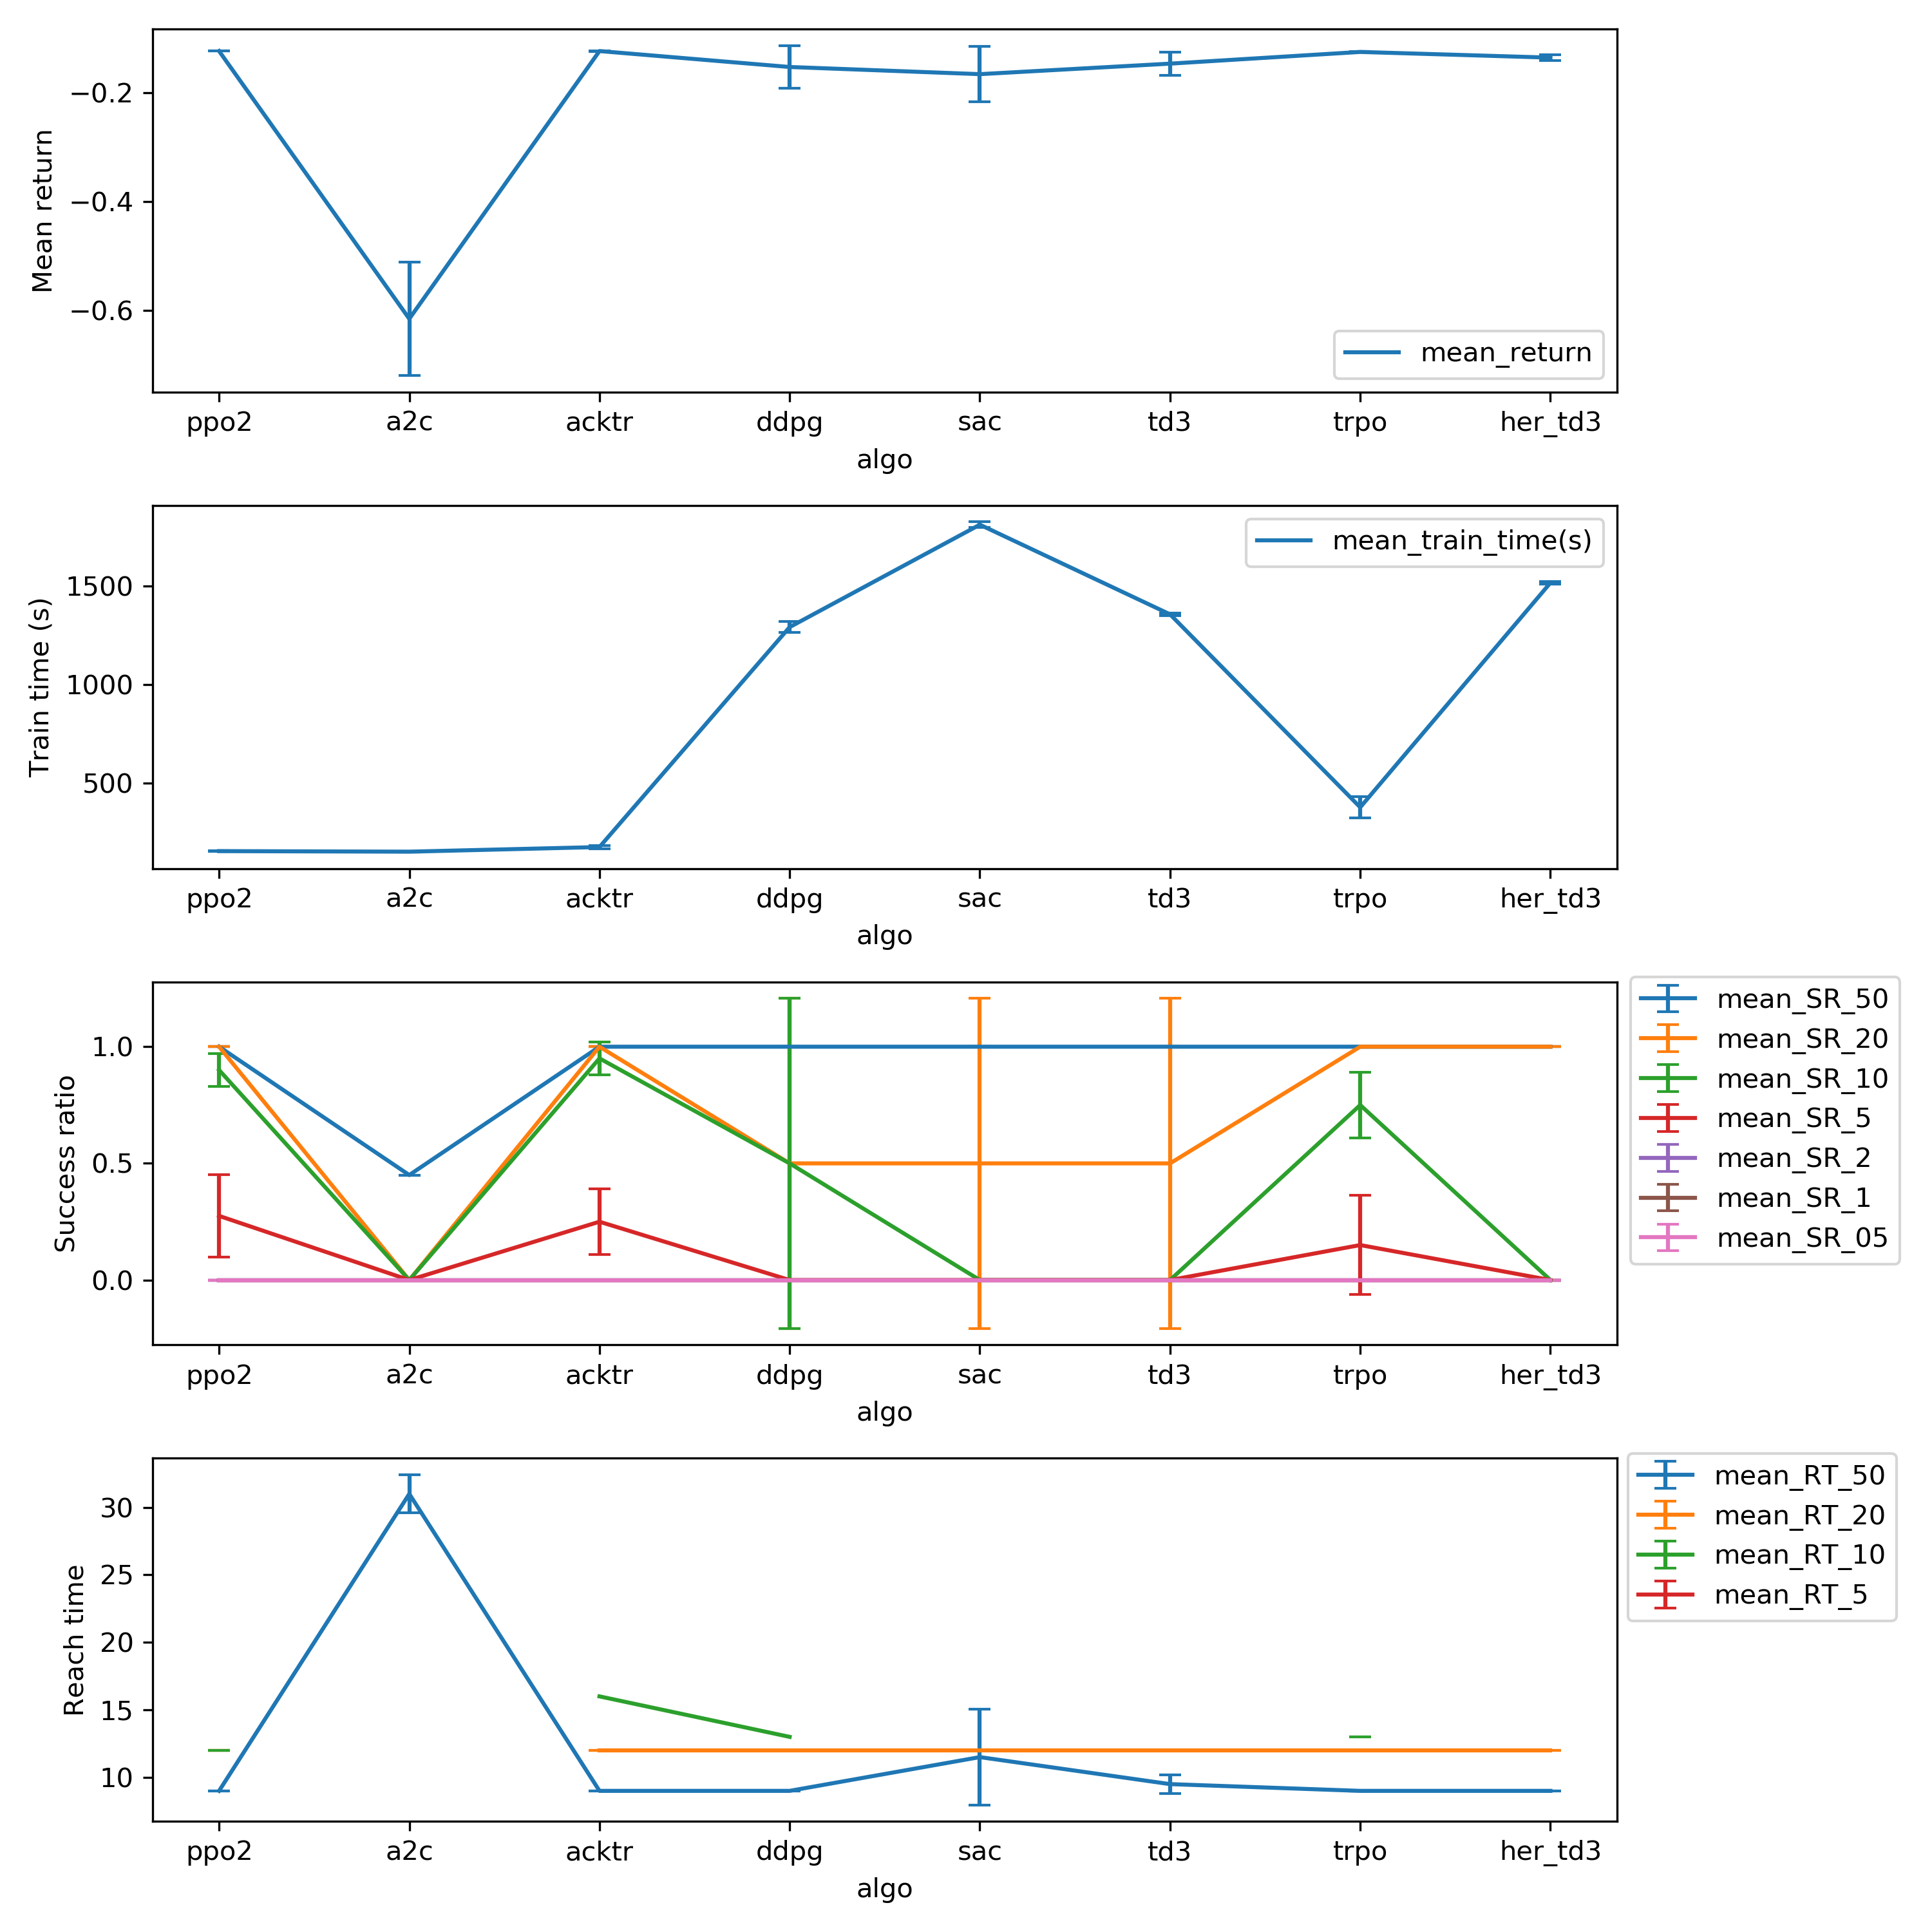
\includegraphics[width=\textwidth]{../algo.png}
\caption{Algorithms applied to widowx-reacher-v5}
\end{figure}

PPO2 gives the best performance and train time.


\section{Manual hyperparameter tuning}

We train with PPO2 and change the hyperparameters. The training environment is:

\begin{itemize}
  \item Environment: widowx-reacher-v5
  \item 6 joints
  \item Fixed goal
  \item Dense reward: -dist**2
\end{itemize}




\begin{figure}[H]
    \centering
    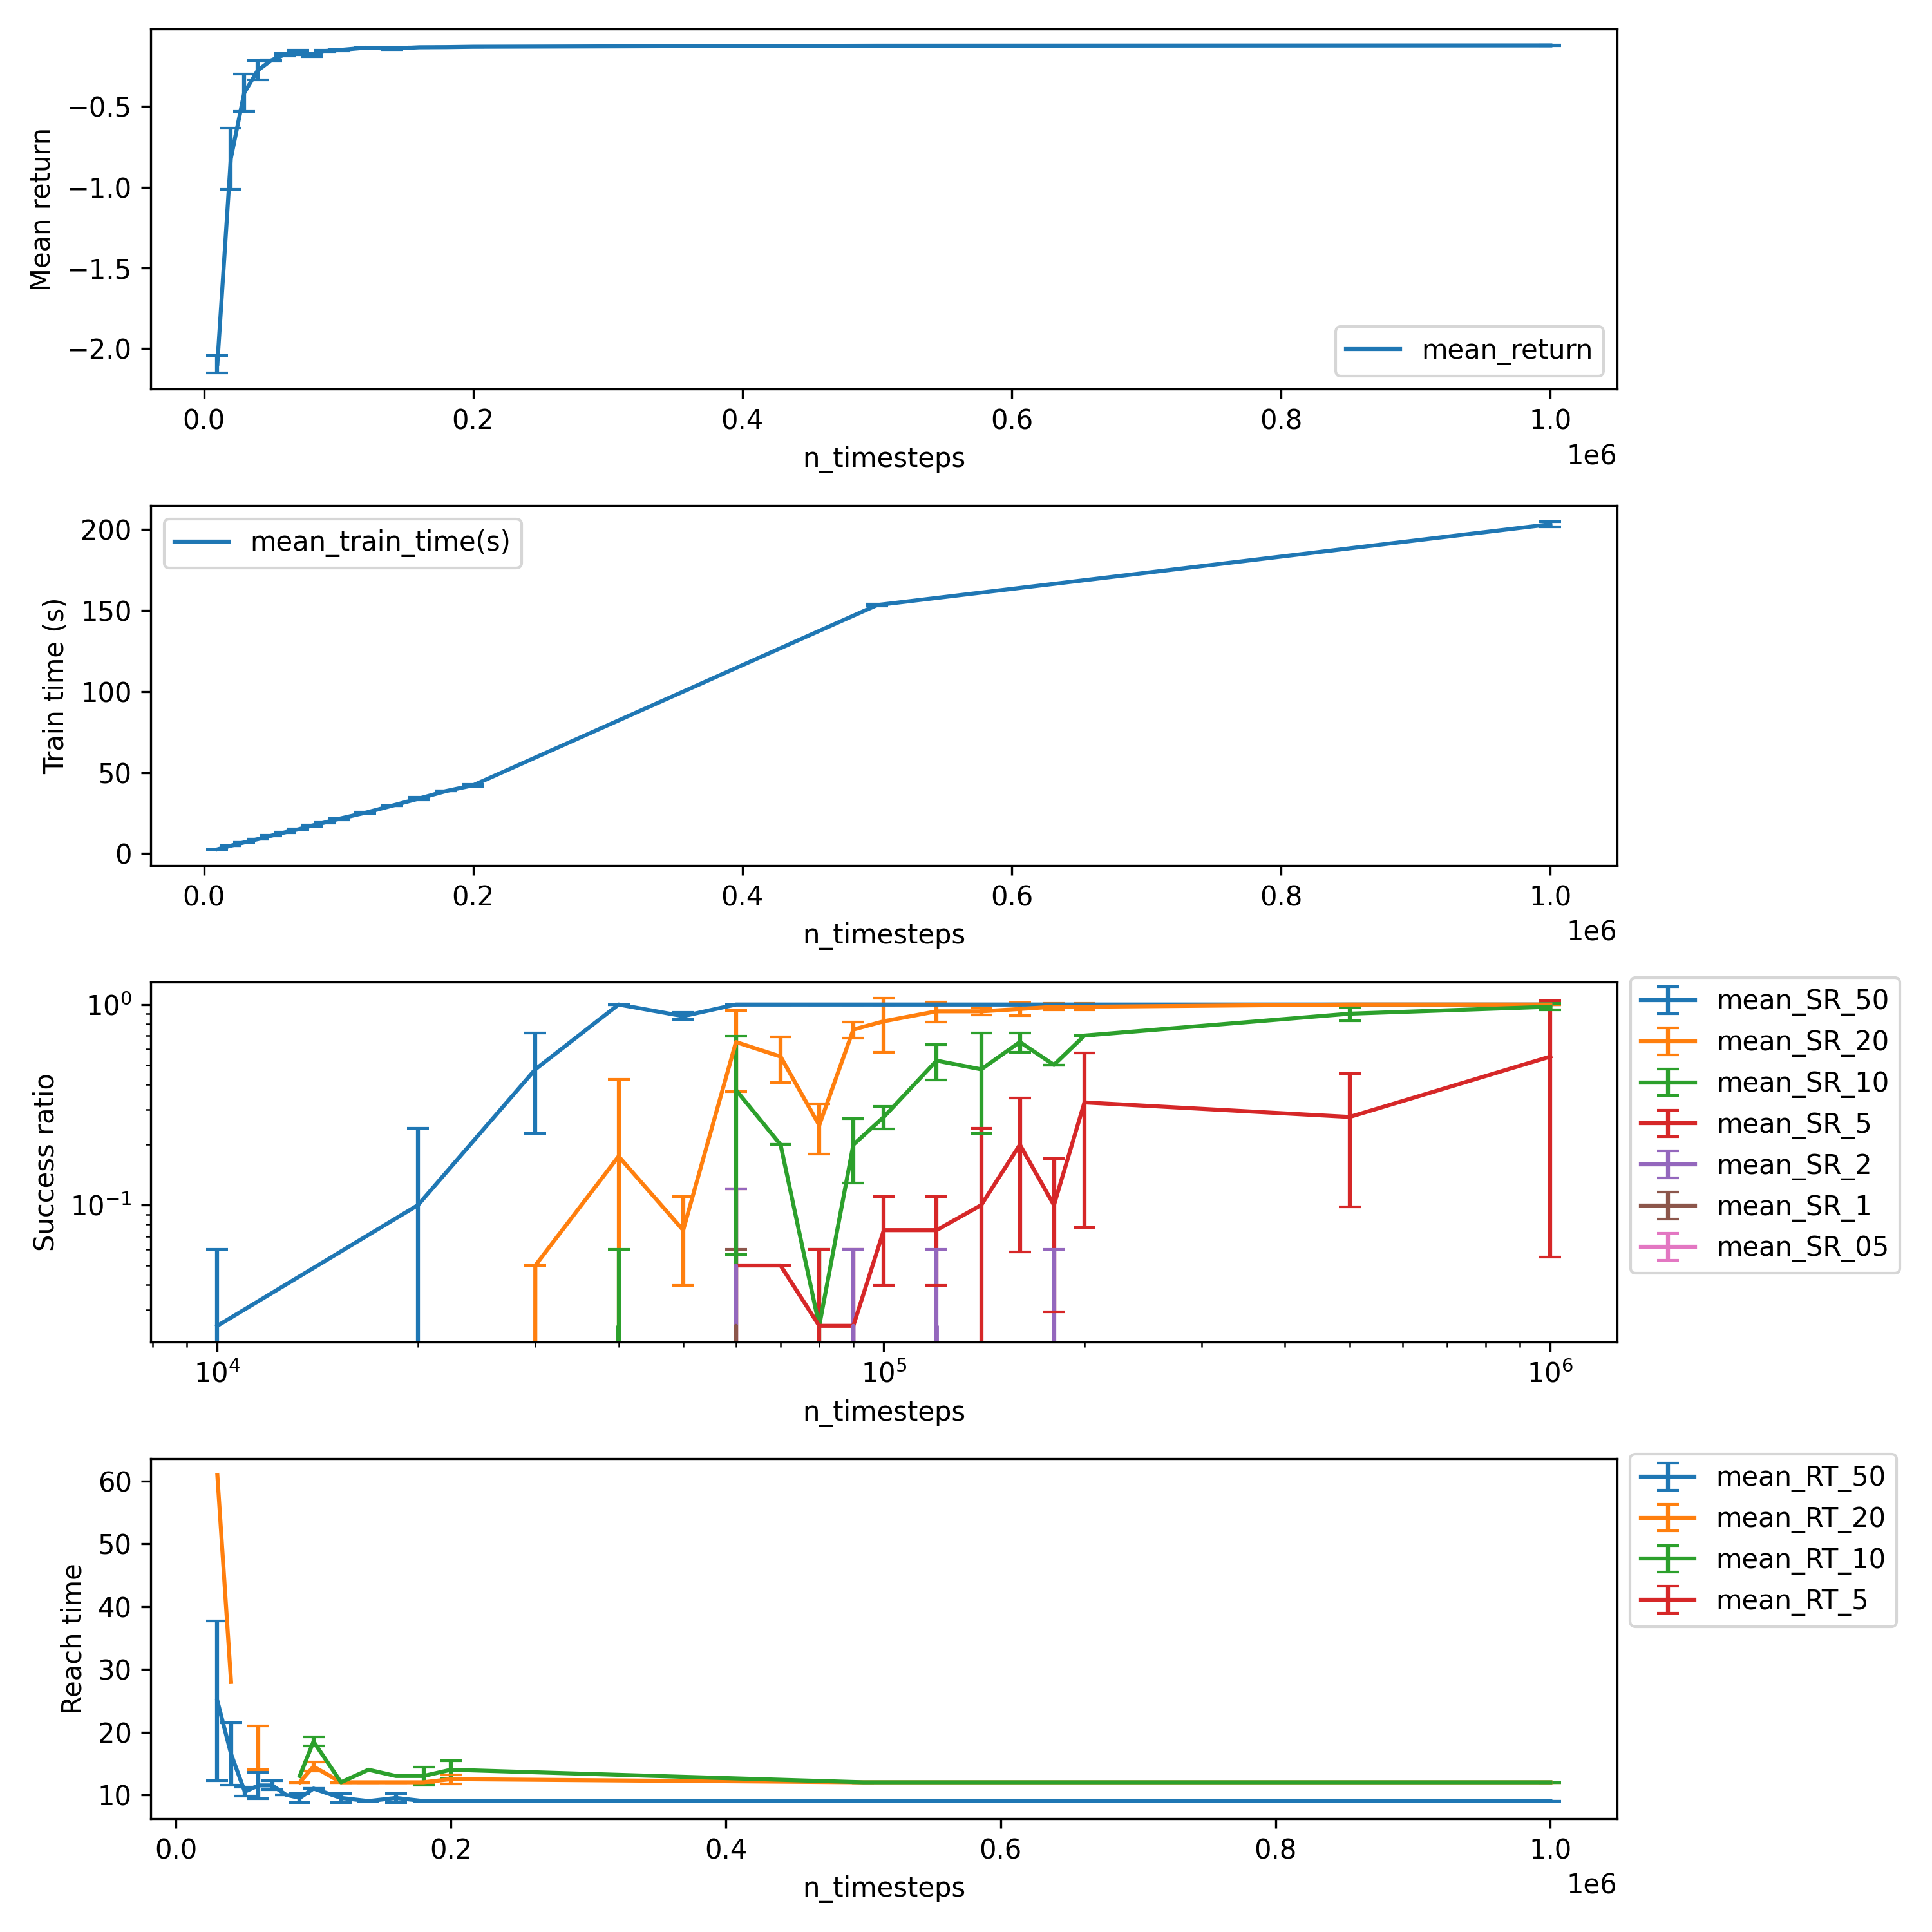
\includegraphics[width=\textwidth]{../ppo2_n_timesteps.png}
\caption{Number of training steps}
\end{figure}


\begin{figure}[H]
    \centering
    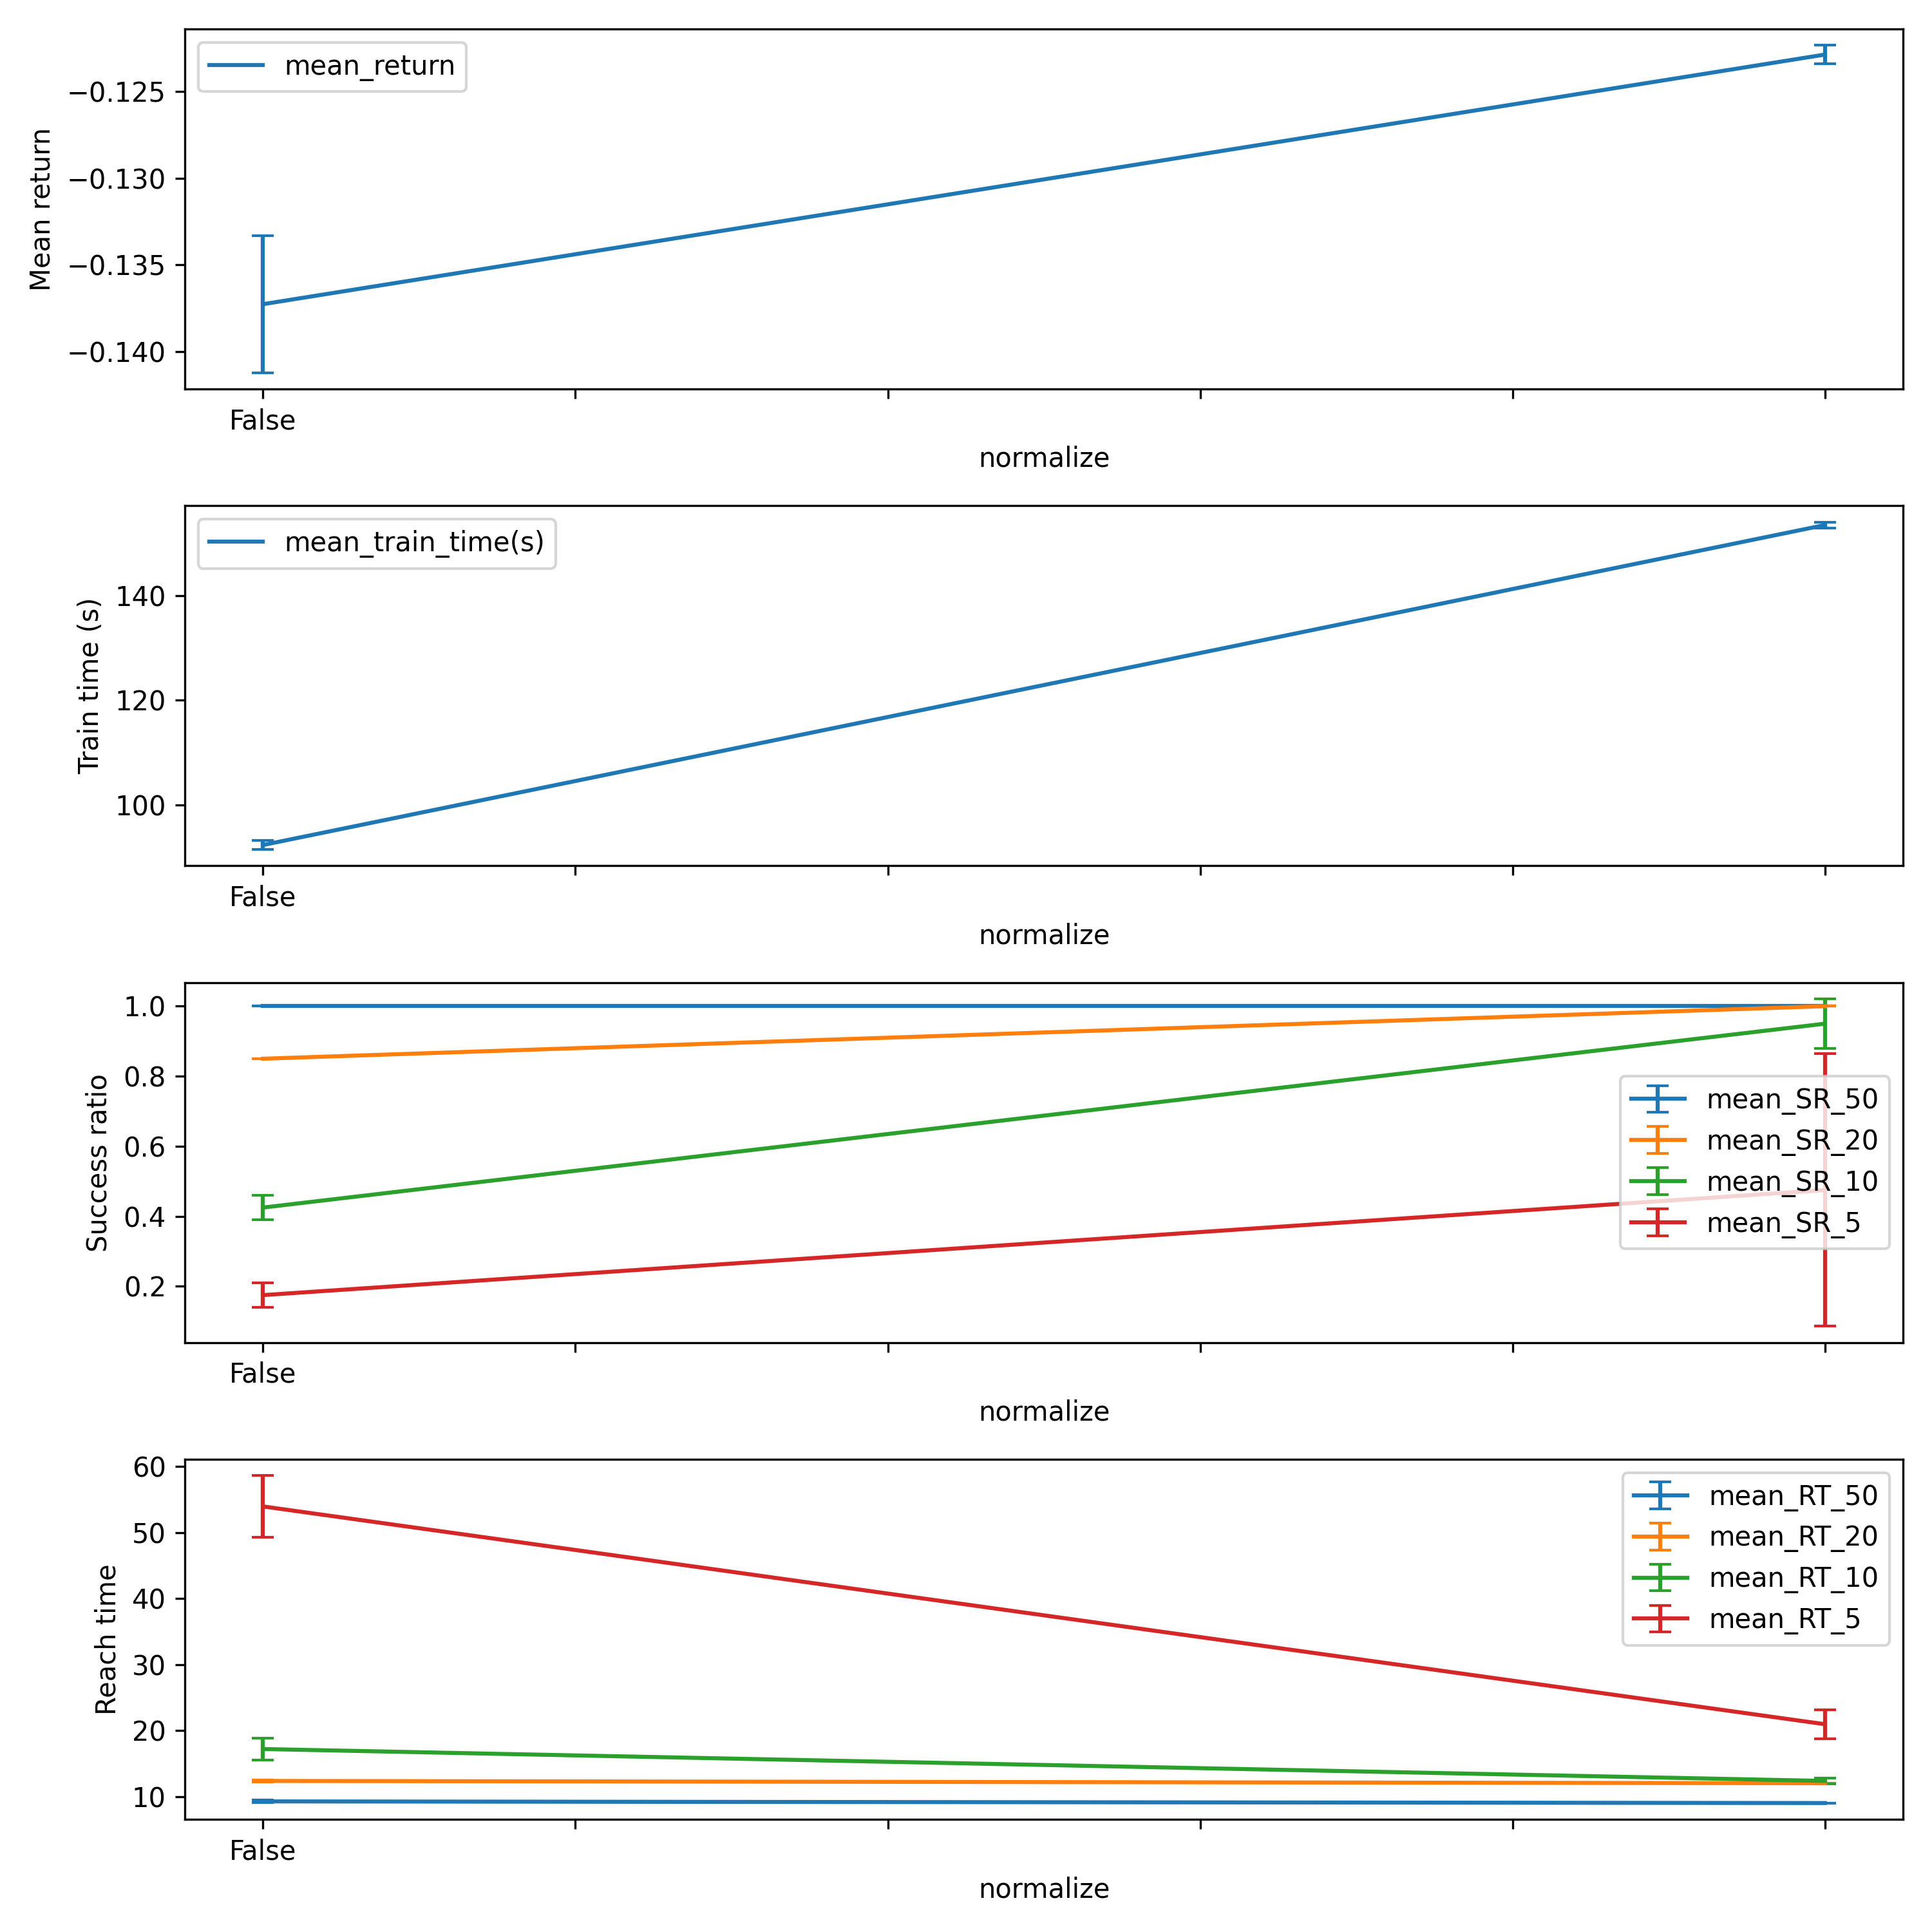
\includegraphics[width=\textwidth]{../ppo2_normalize.png}
\caption{Normalise observation and reward}
\end{figure}

\begin{figure}[H]
    \centering
    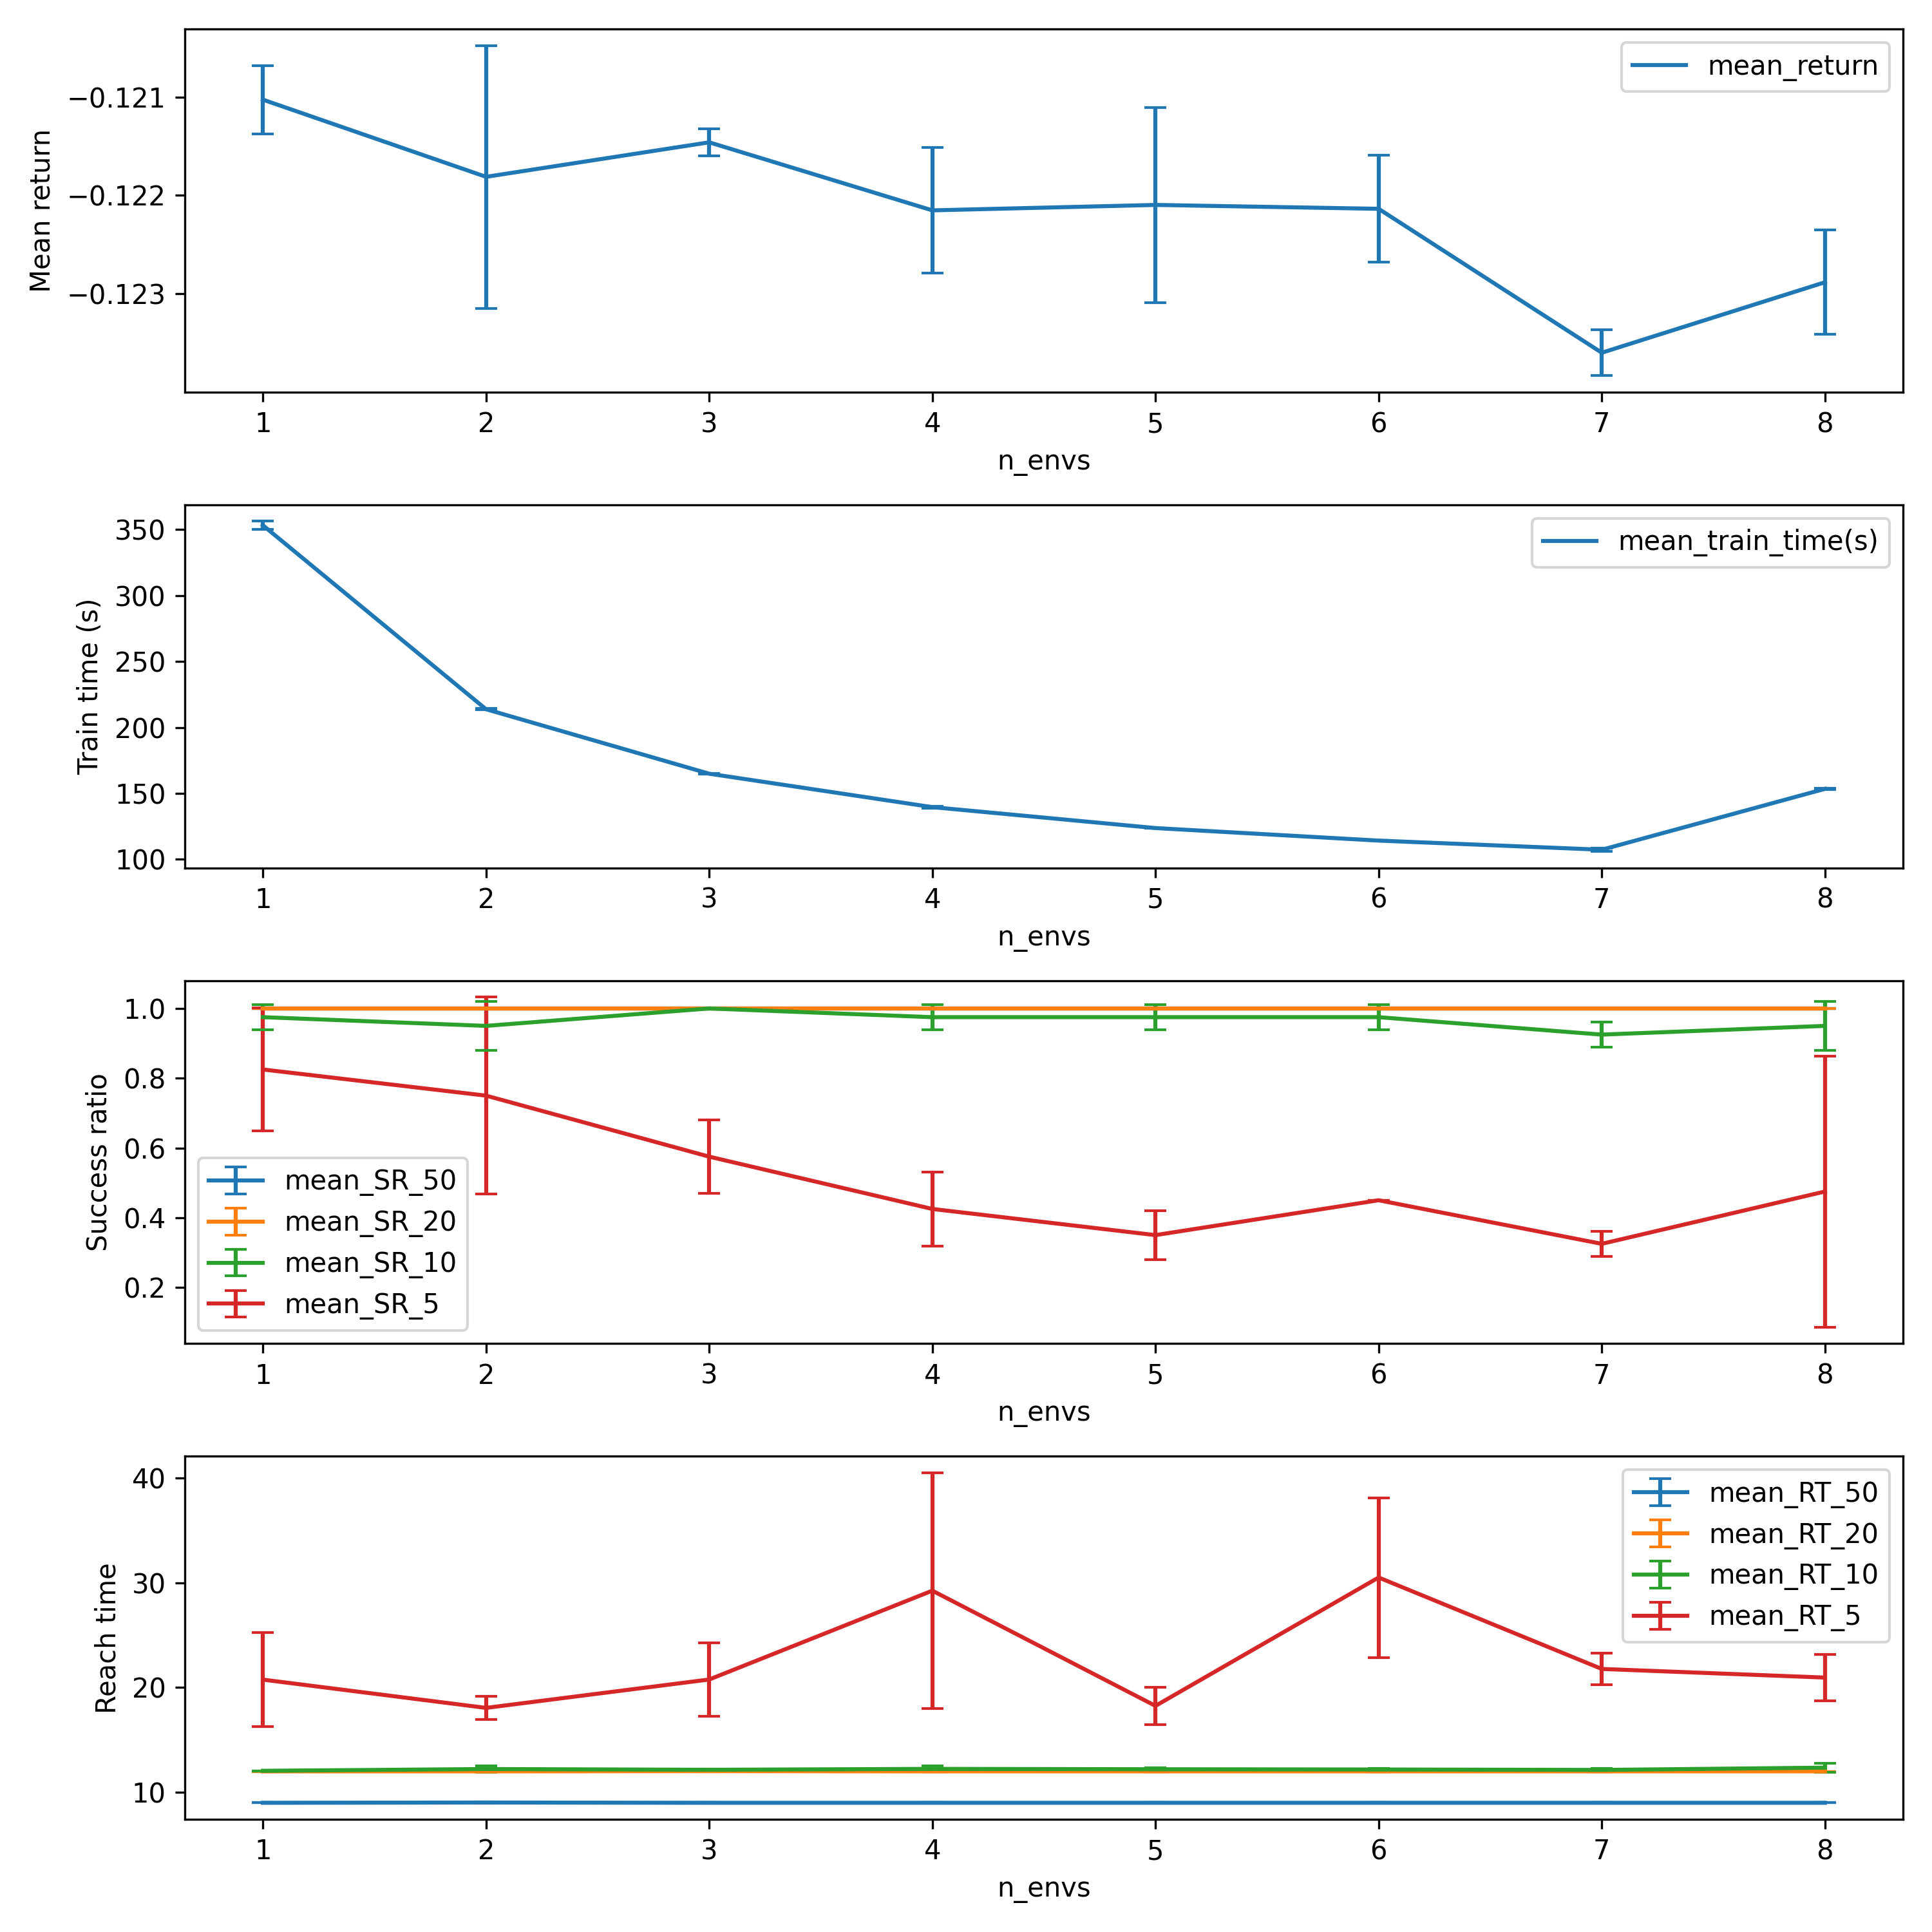
\includegraphics[width=\textwidth]{../ppo2_n_envs.png}
\caption{Number of parallel environments}
\end{figure}

\begin{figure}[H]
    \centering
    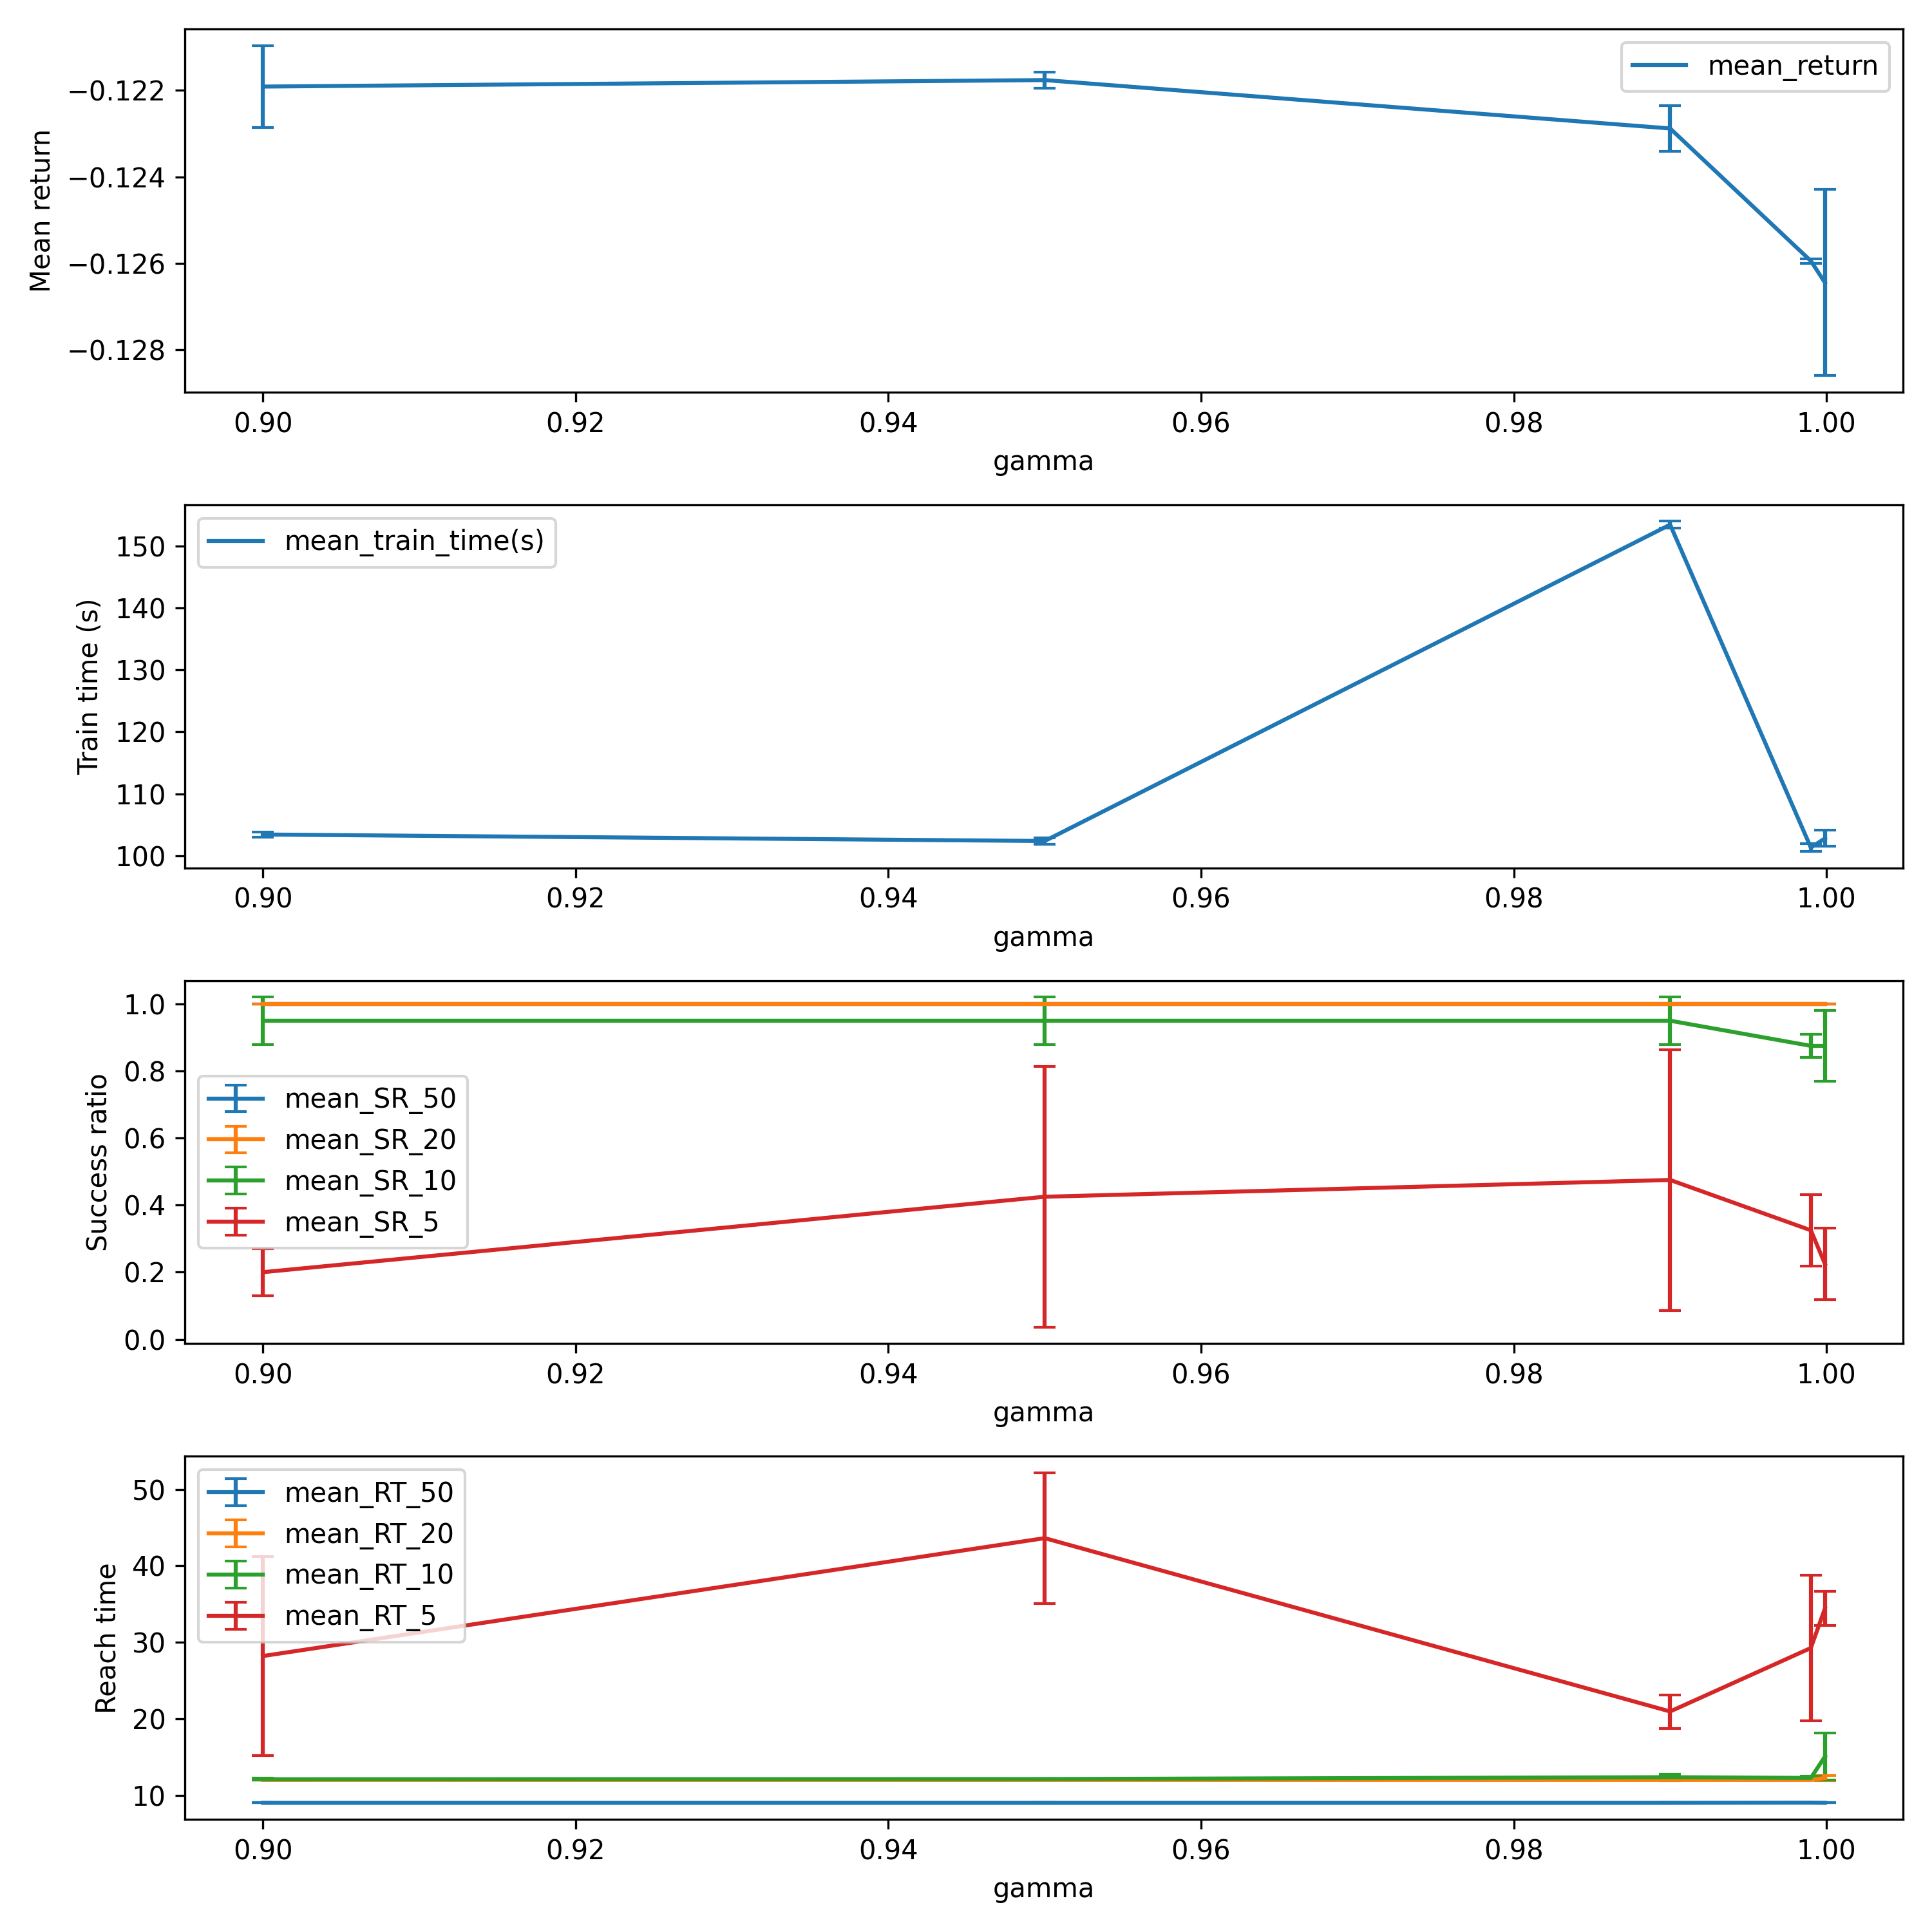
\includegraphics[width=\textwidth]{../ppo2_gamma.png}
\caption{Gamma}
\end{figure}

\begin{figure}[H]
    \centering
    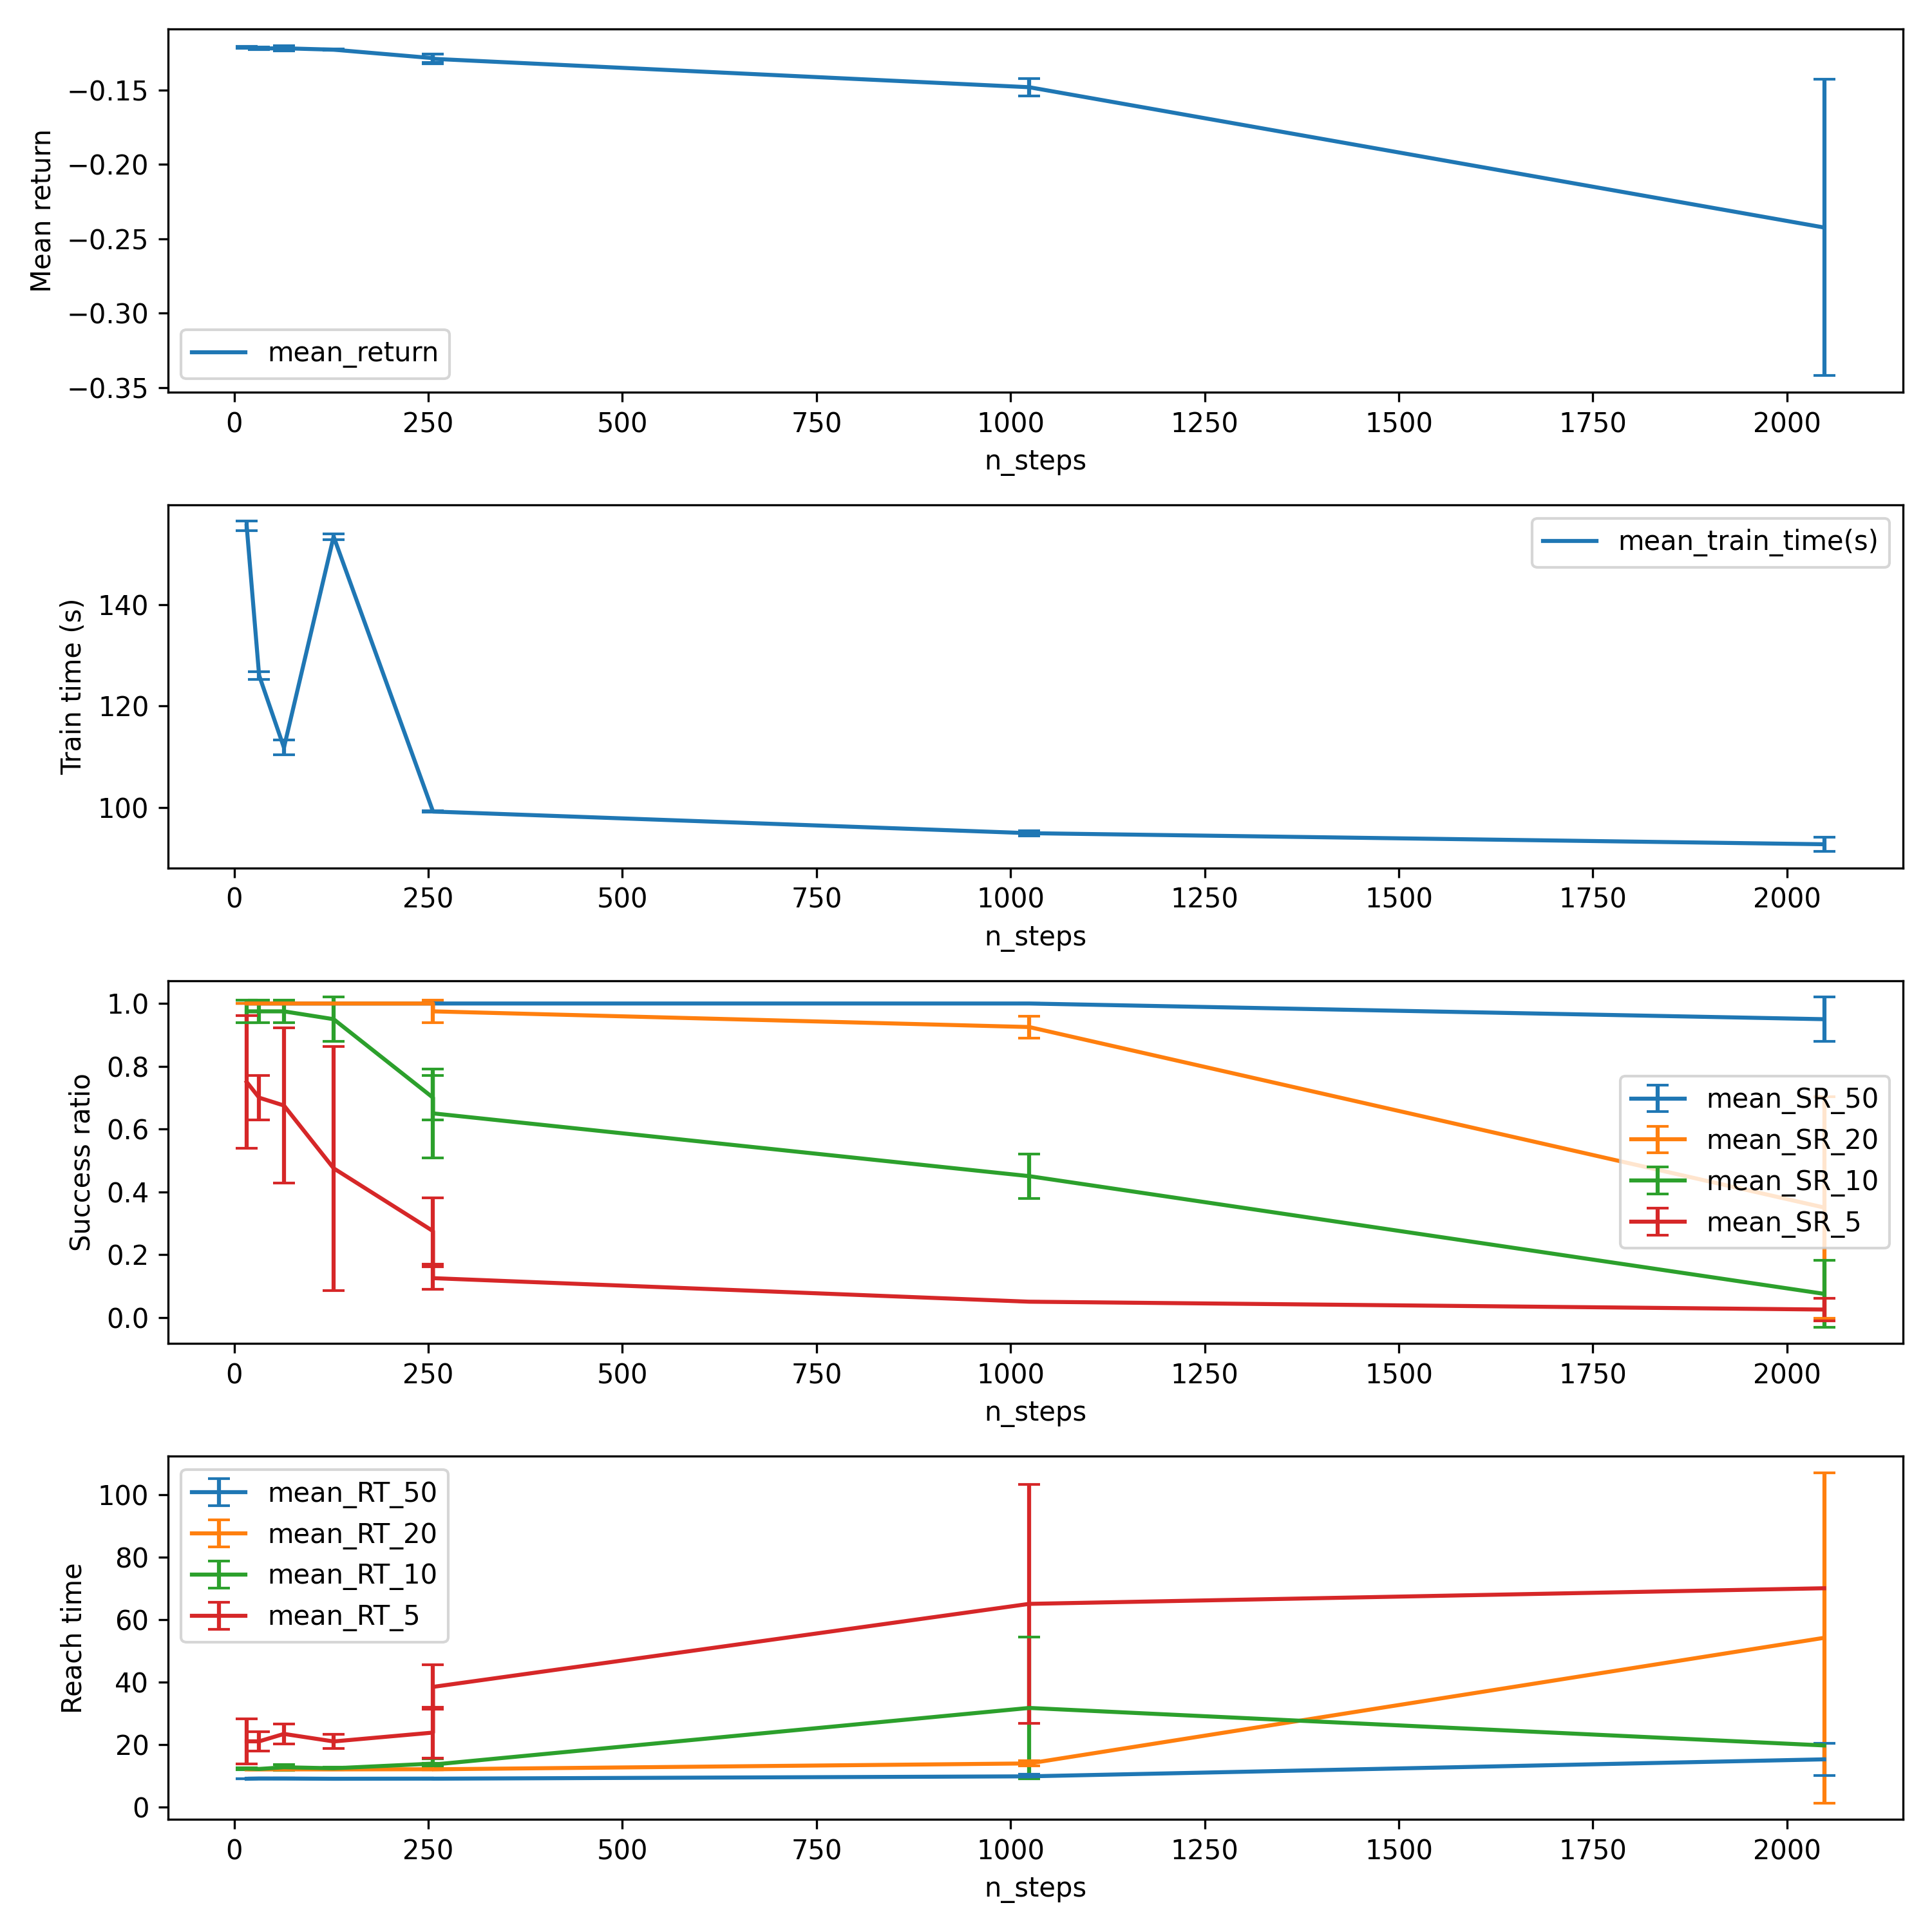
\includegraphics[width=\textwidth]{../ppo2_n_steps.png}
\caption{Number of steps to run for each environment per update}
\end{figure}

\begin{figure}[H]
    \centering
    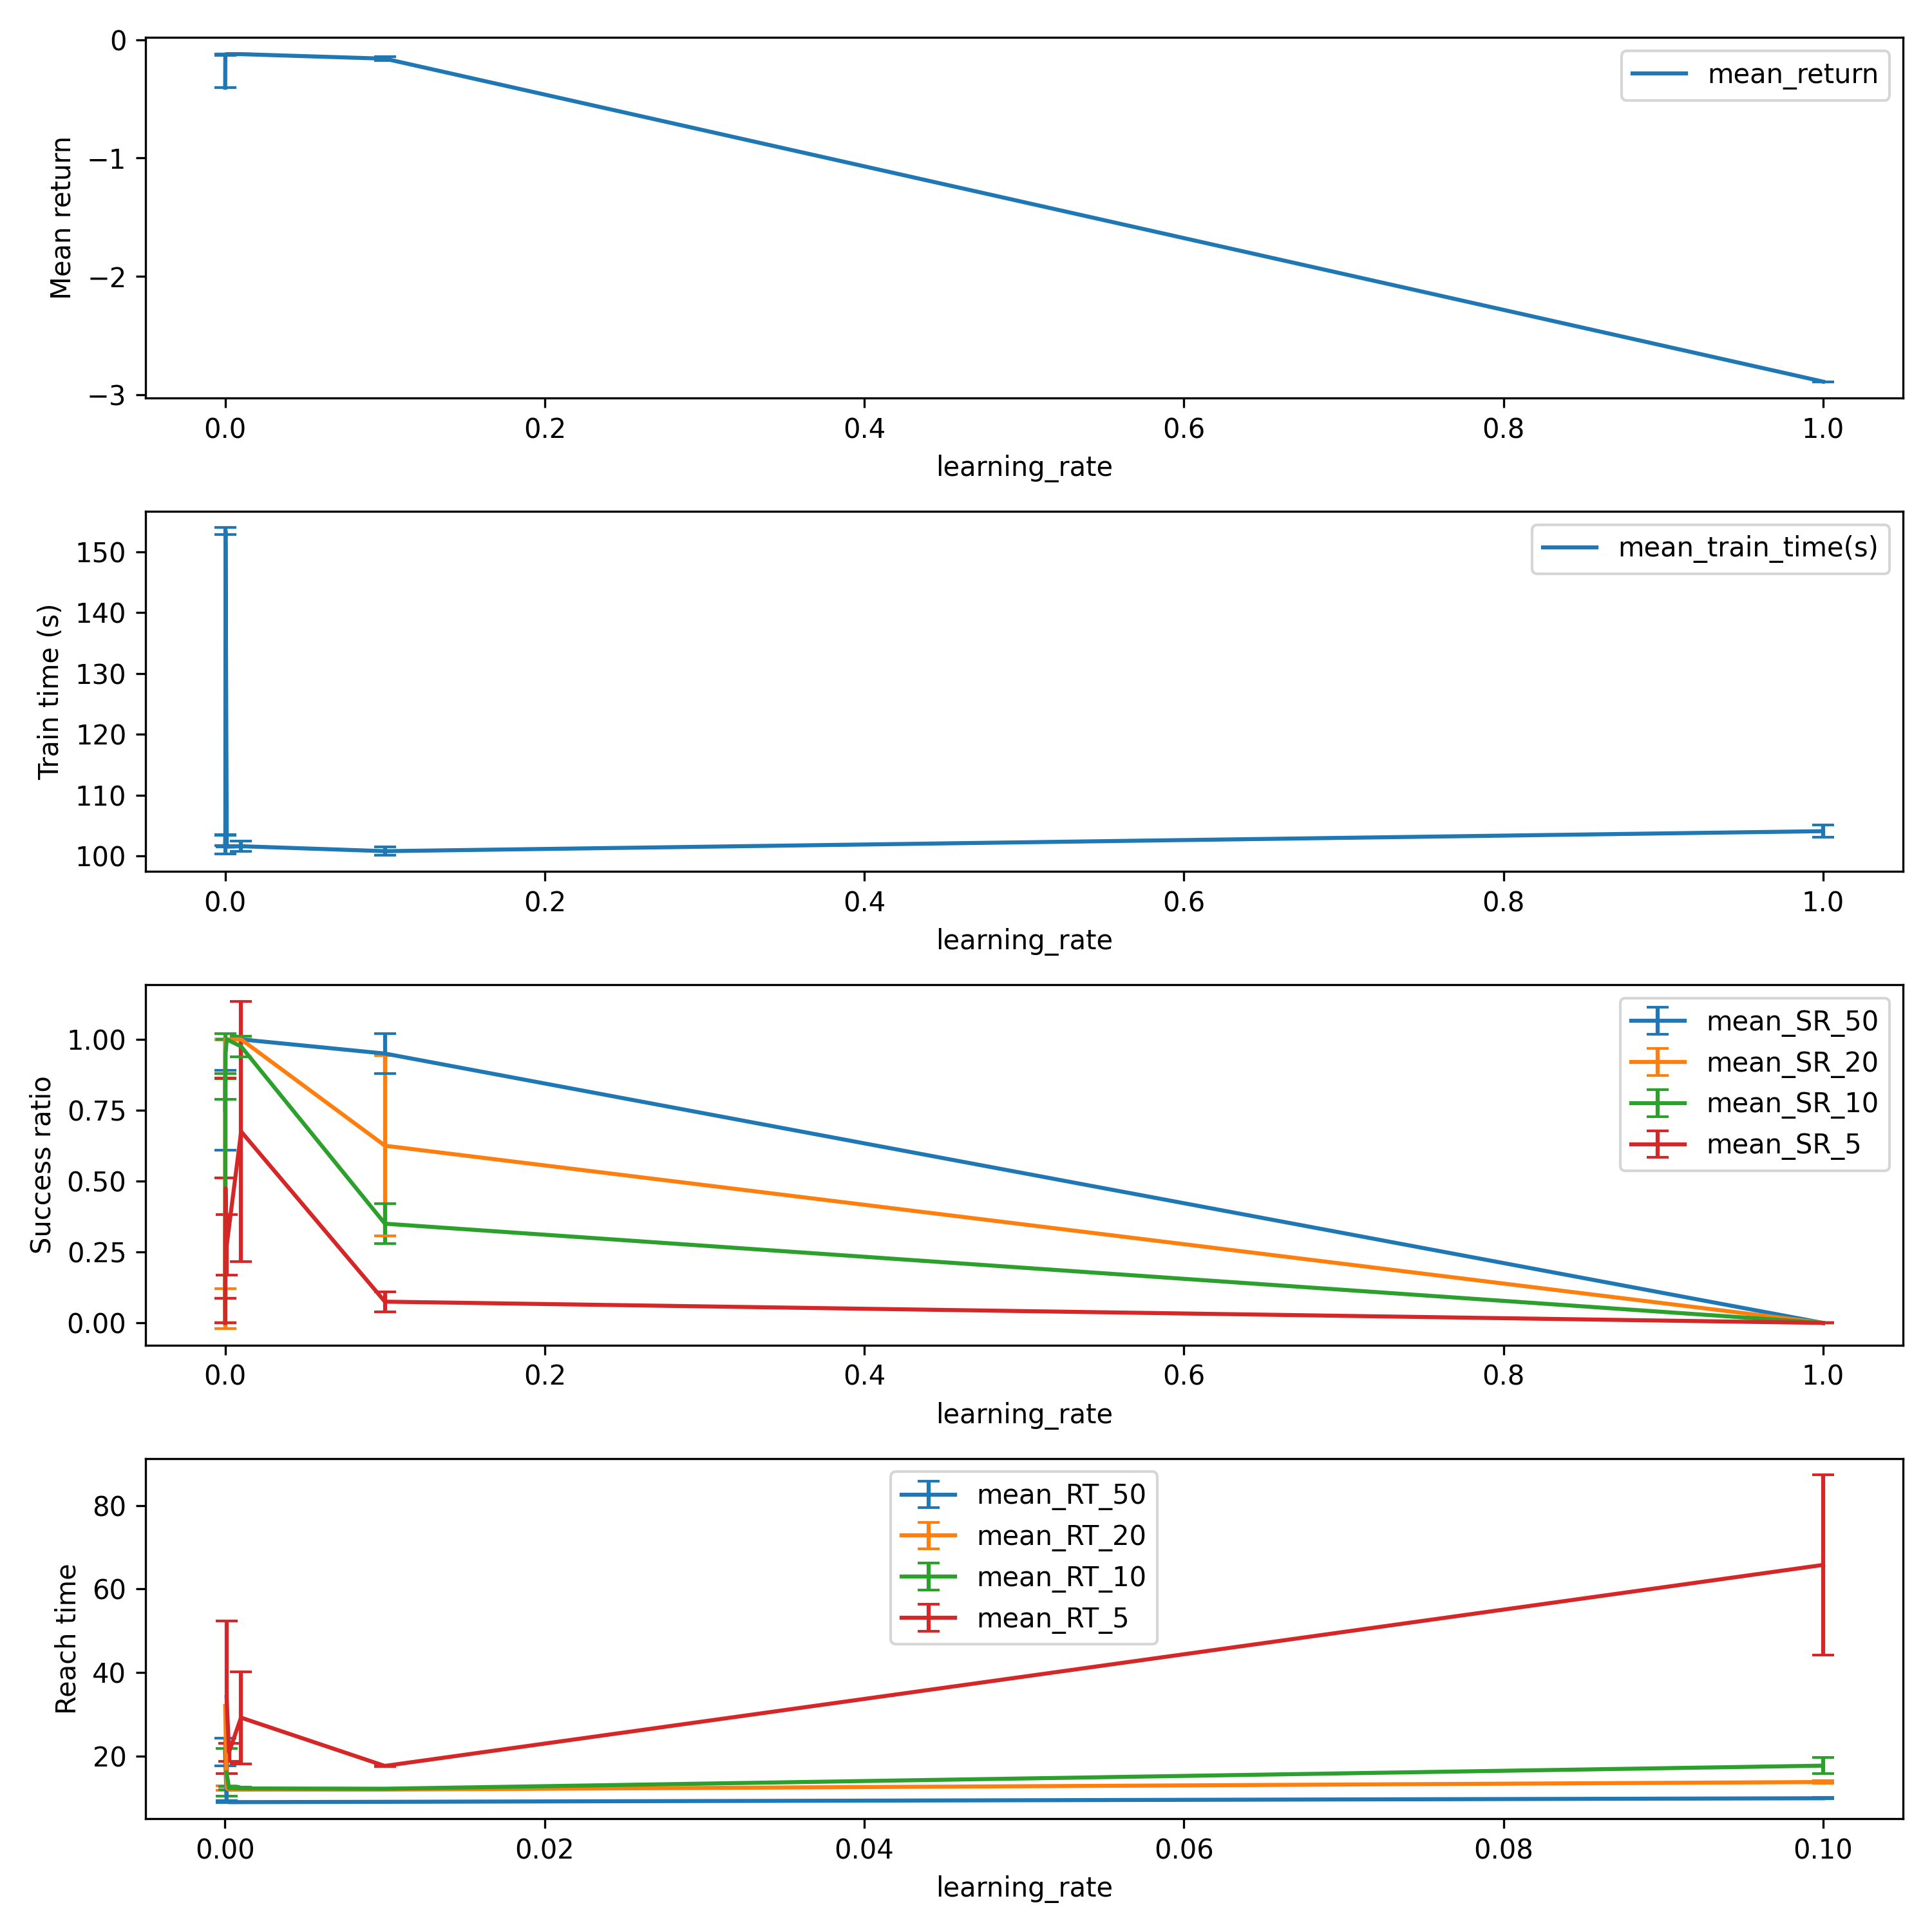
\includegraphics[width=\textwidth]{../ppo2_learning_rate.png}
\caption{Learning rate}
\end{figure}


\begin{figure}[H]
    \centering
    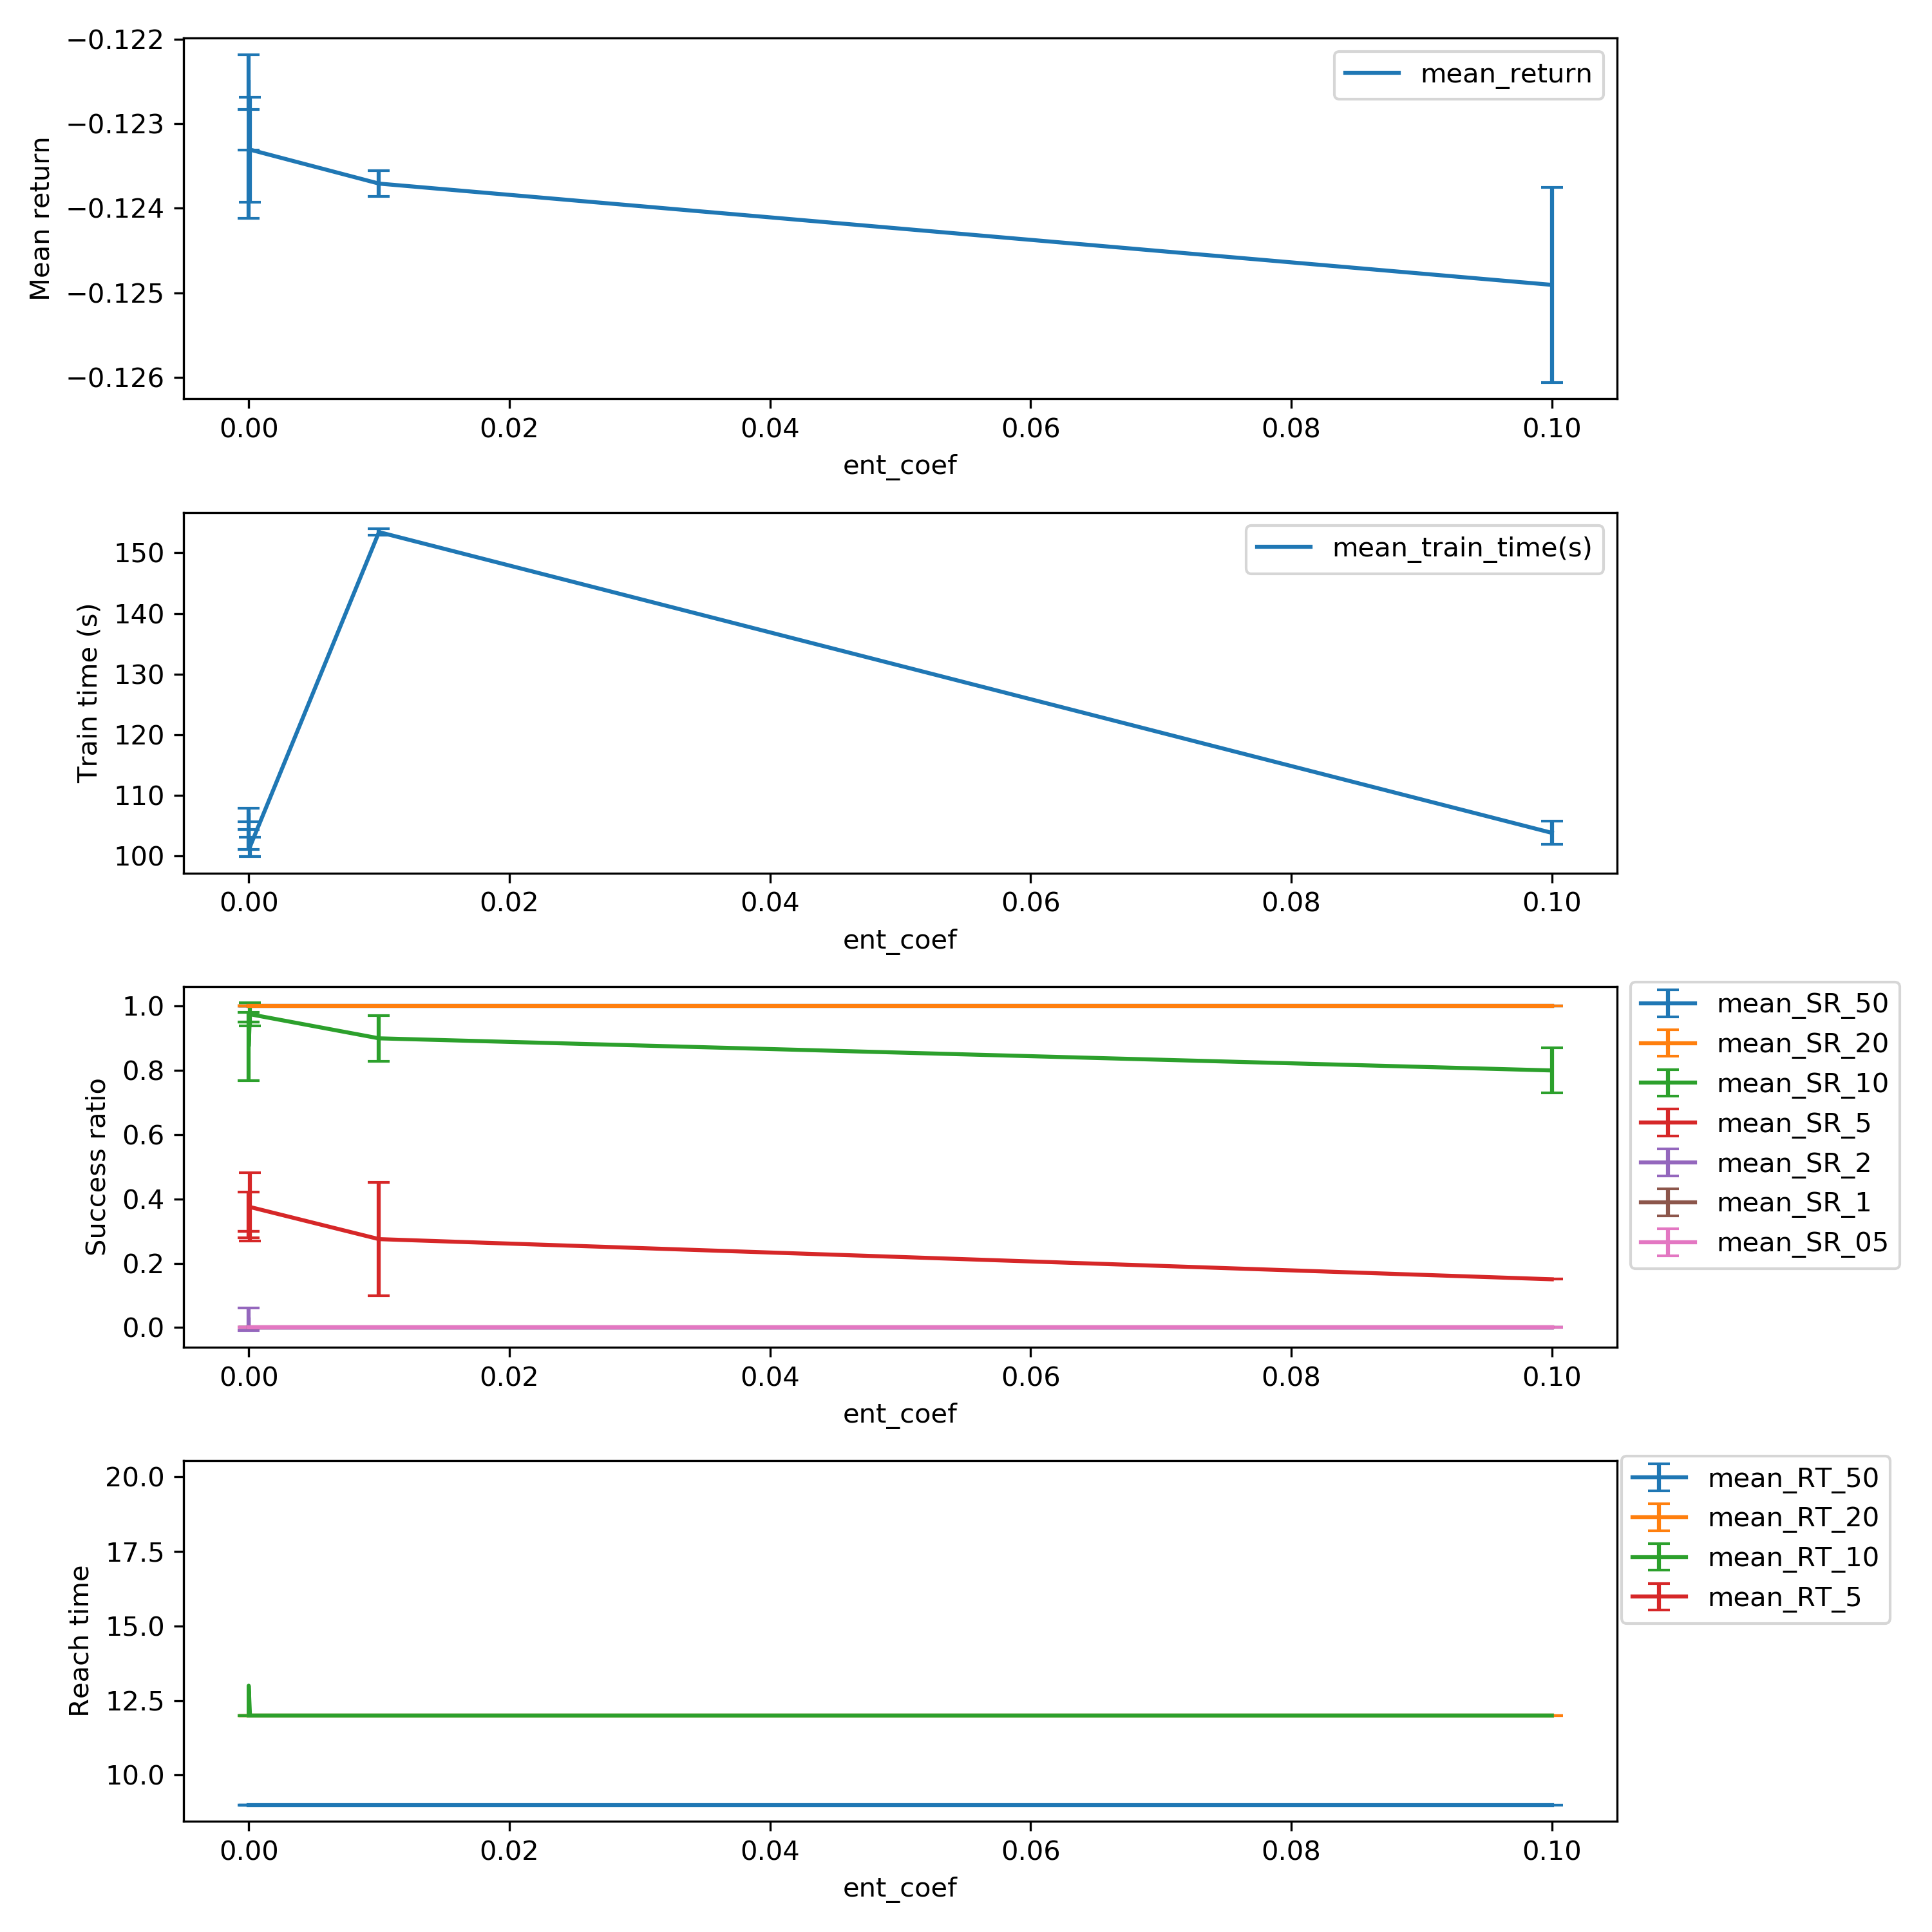
\includegraphics[width=\textwidth]{../ppo2_ent_coef.png}
\caption{Entropy coefficient for the loss calculation}
\end{figure}


\begin{figure}[H]
    \centering
    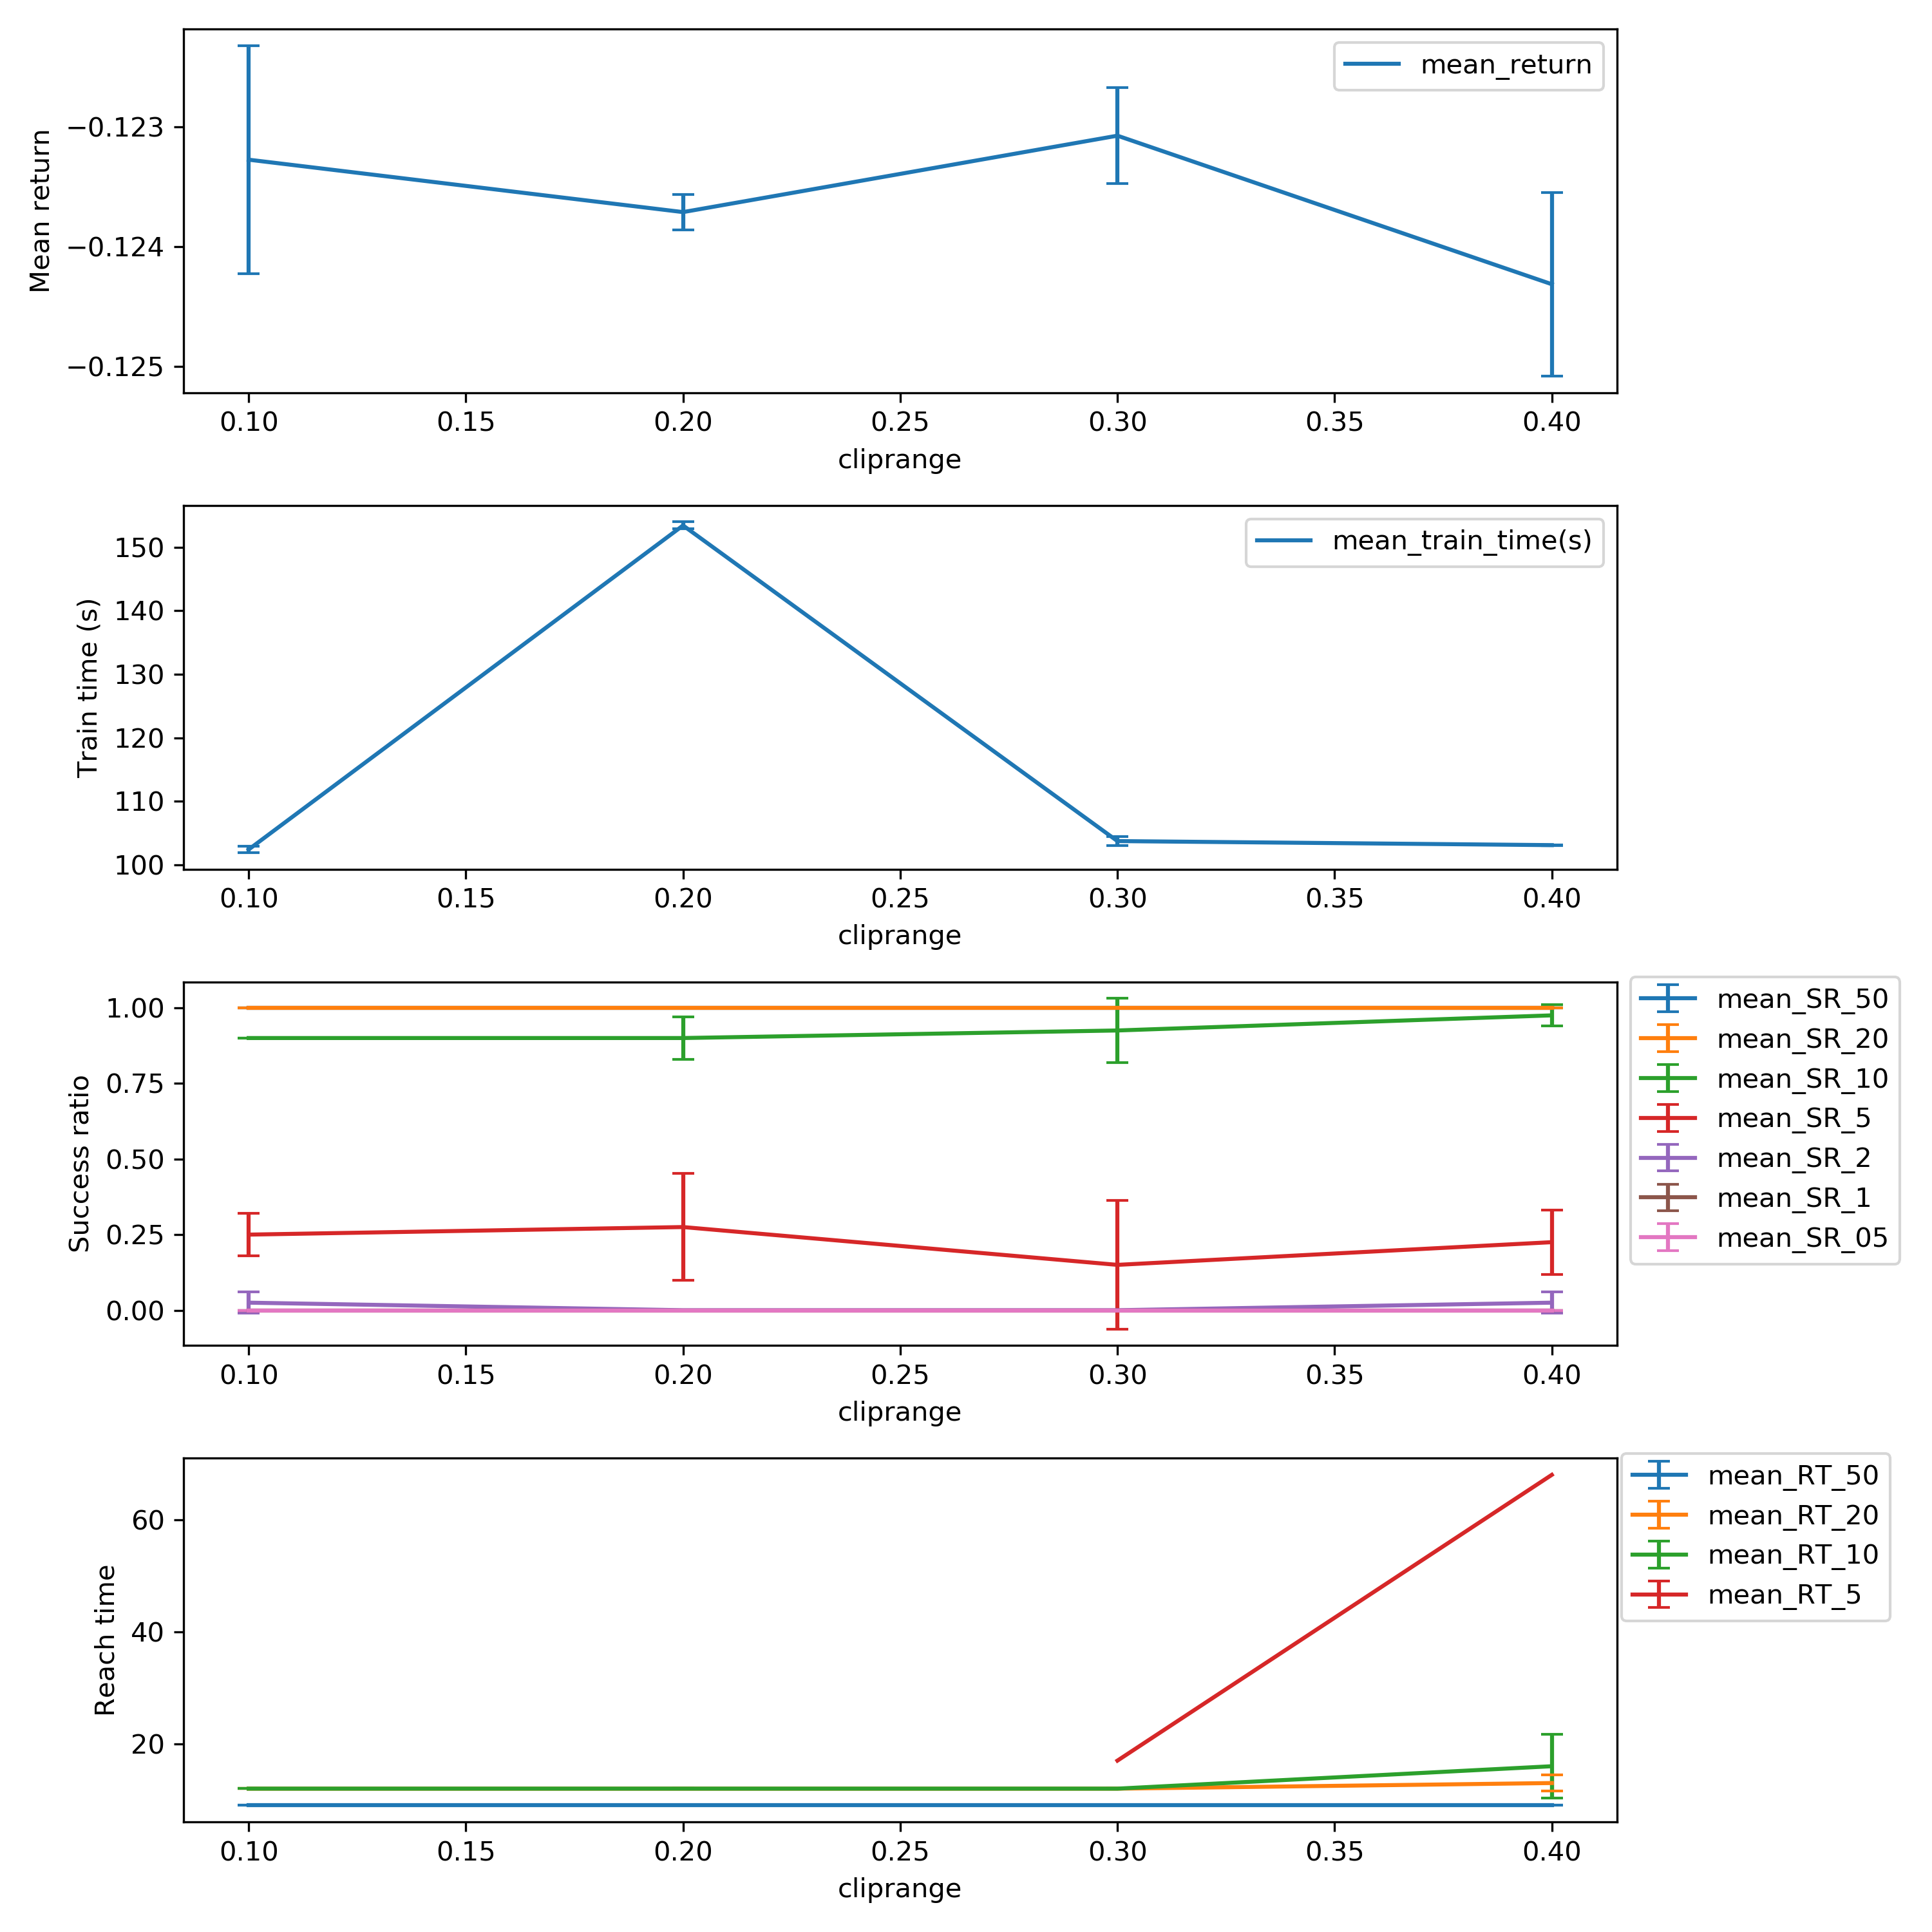
\includegraphics[width=\textwidth]{../ppo2_cliprange.png}
\caption{Clipping parameter}
\end{figure}

\begin{figure}[H]
    \centering
    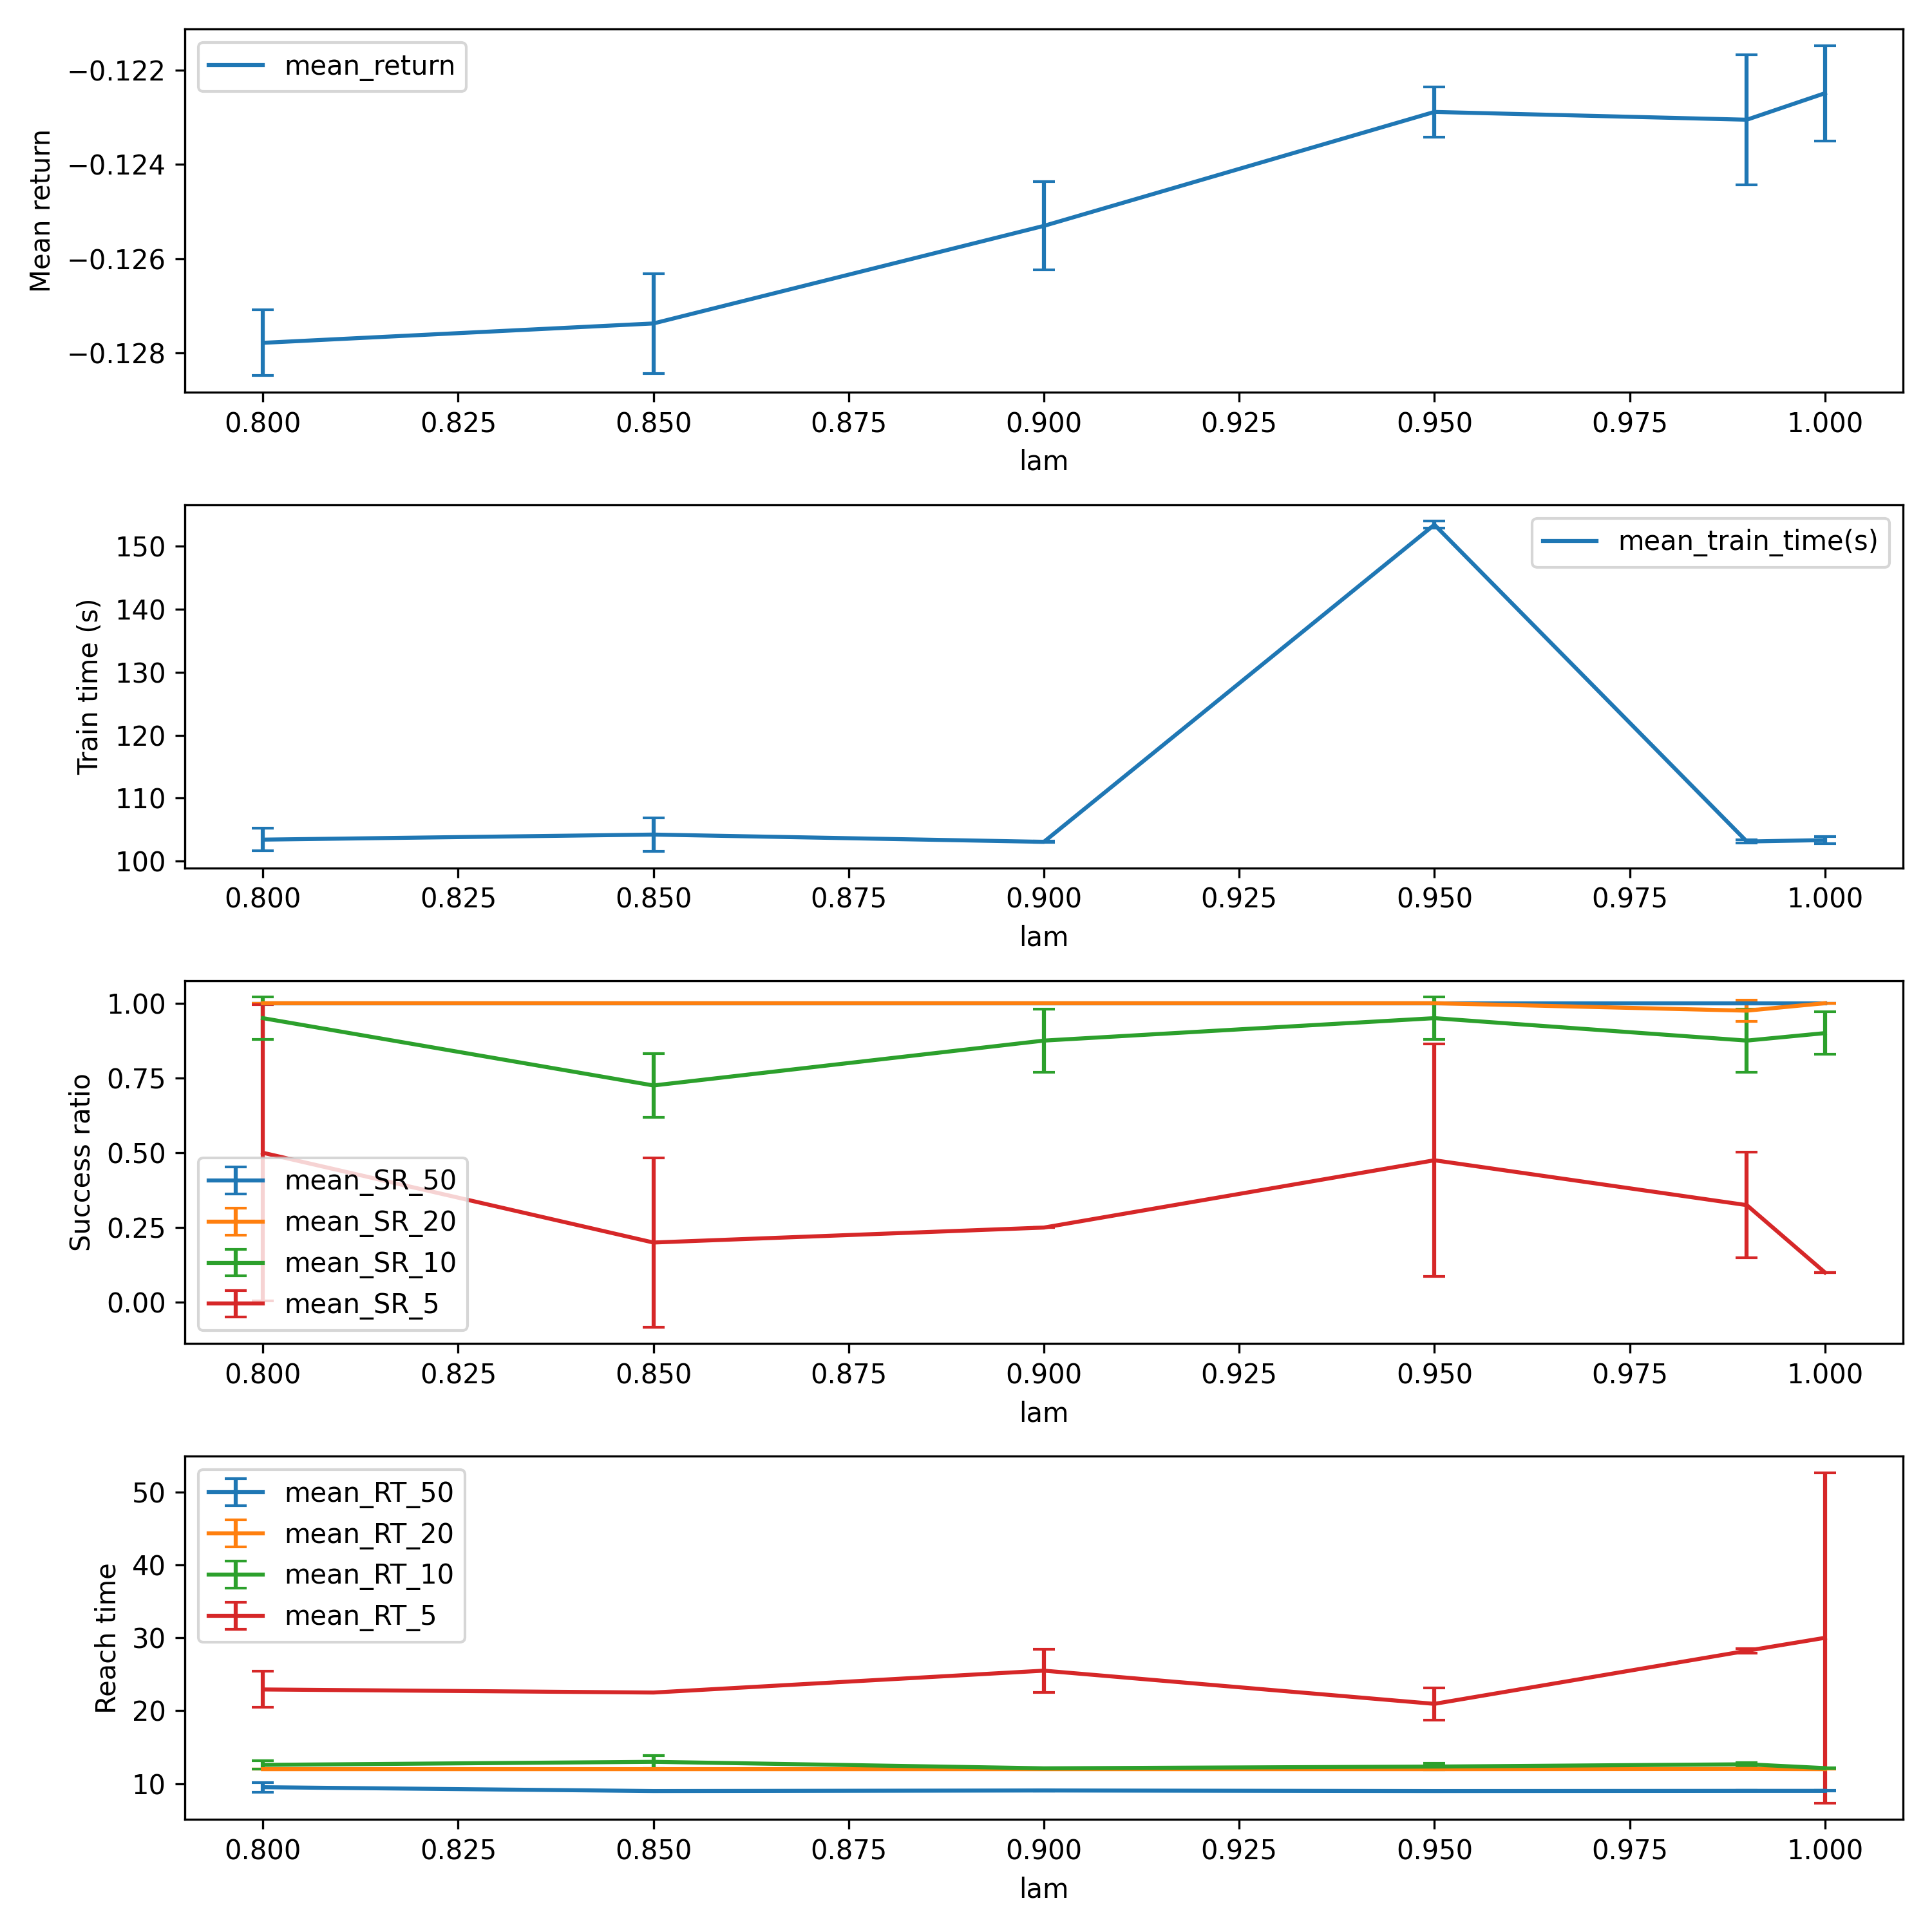
\includegraphics[width=\textwidth]{../ppo2_lam.png}
\caption{Factor for trade-off of bias vs variance for Generalized Advantage Estimator}
\end{figure}

\begin{figure}[H]
    \centering
    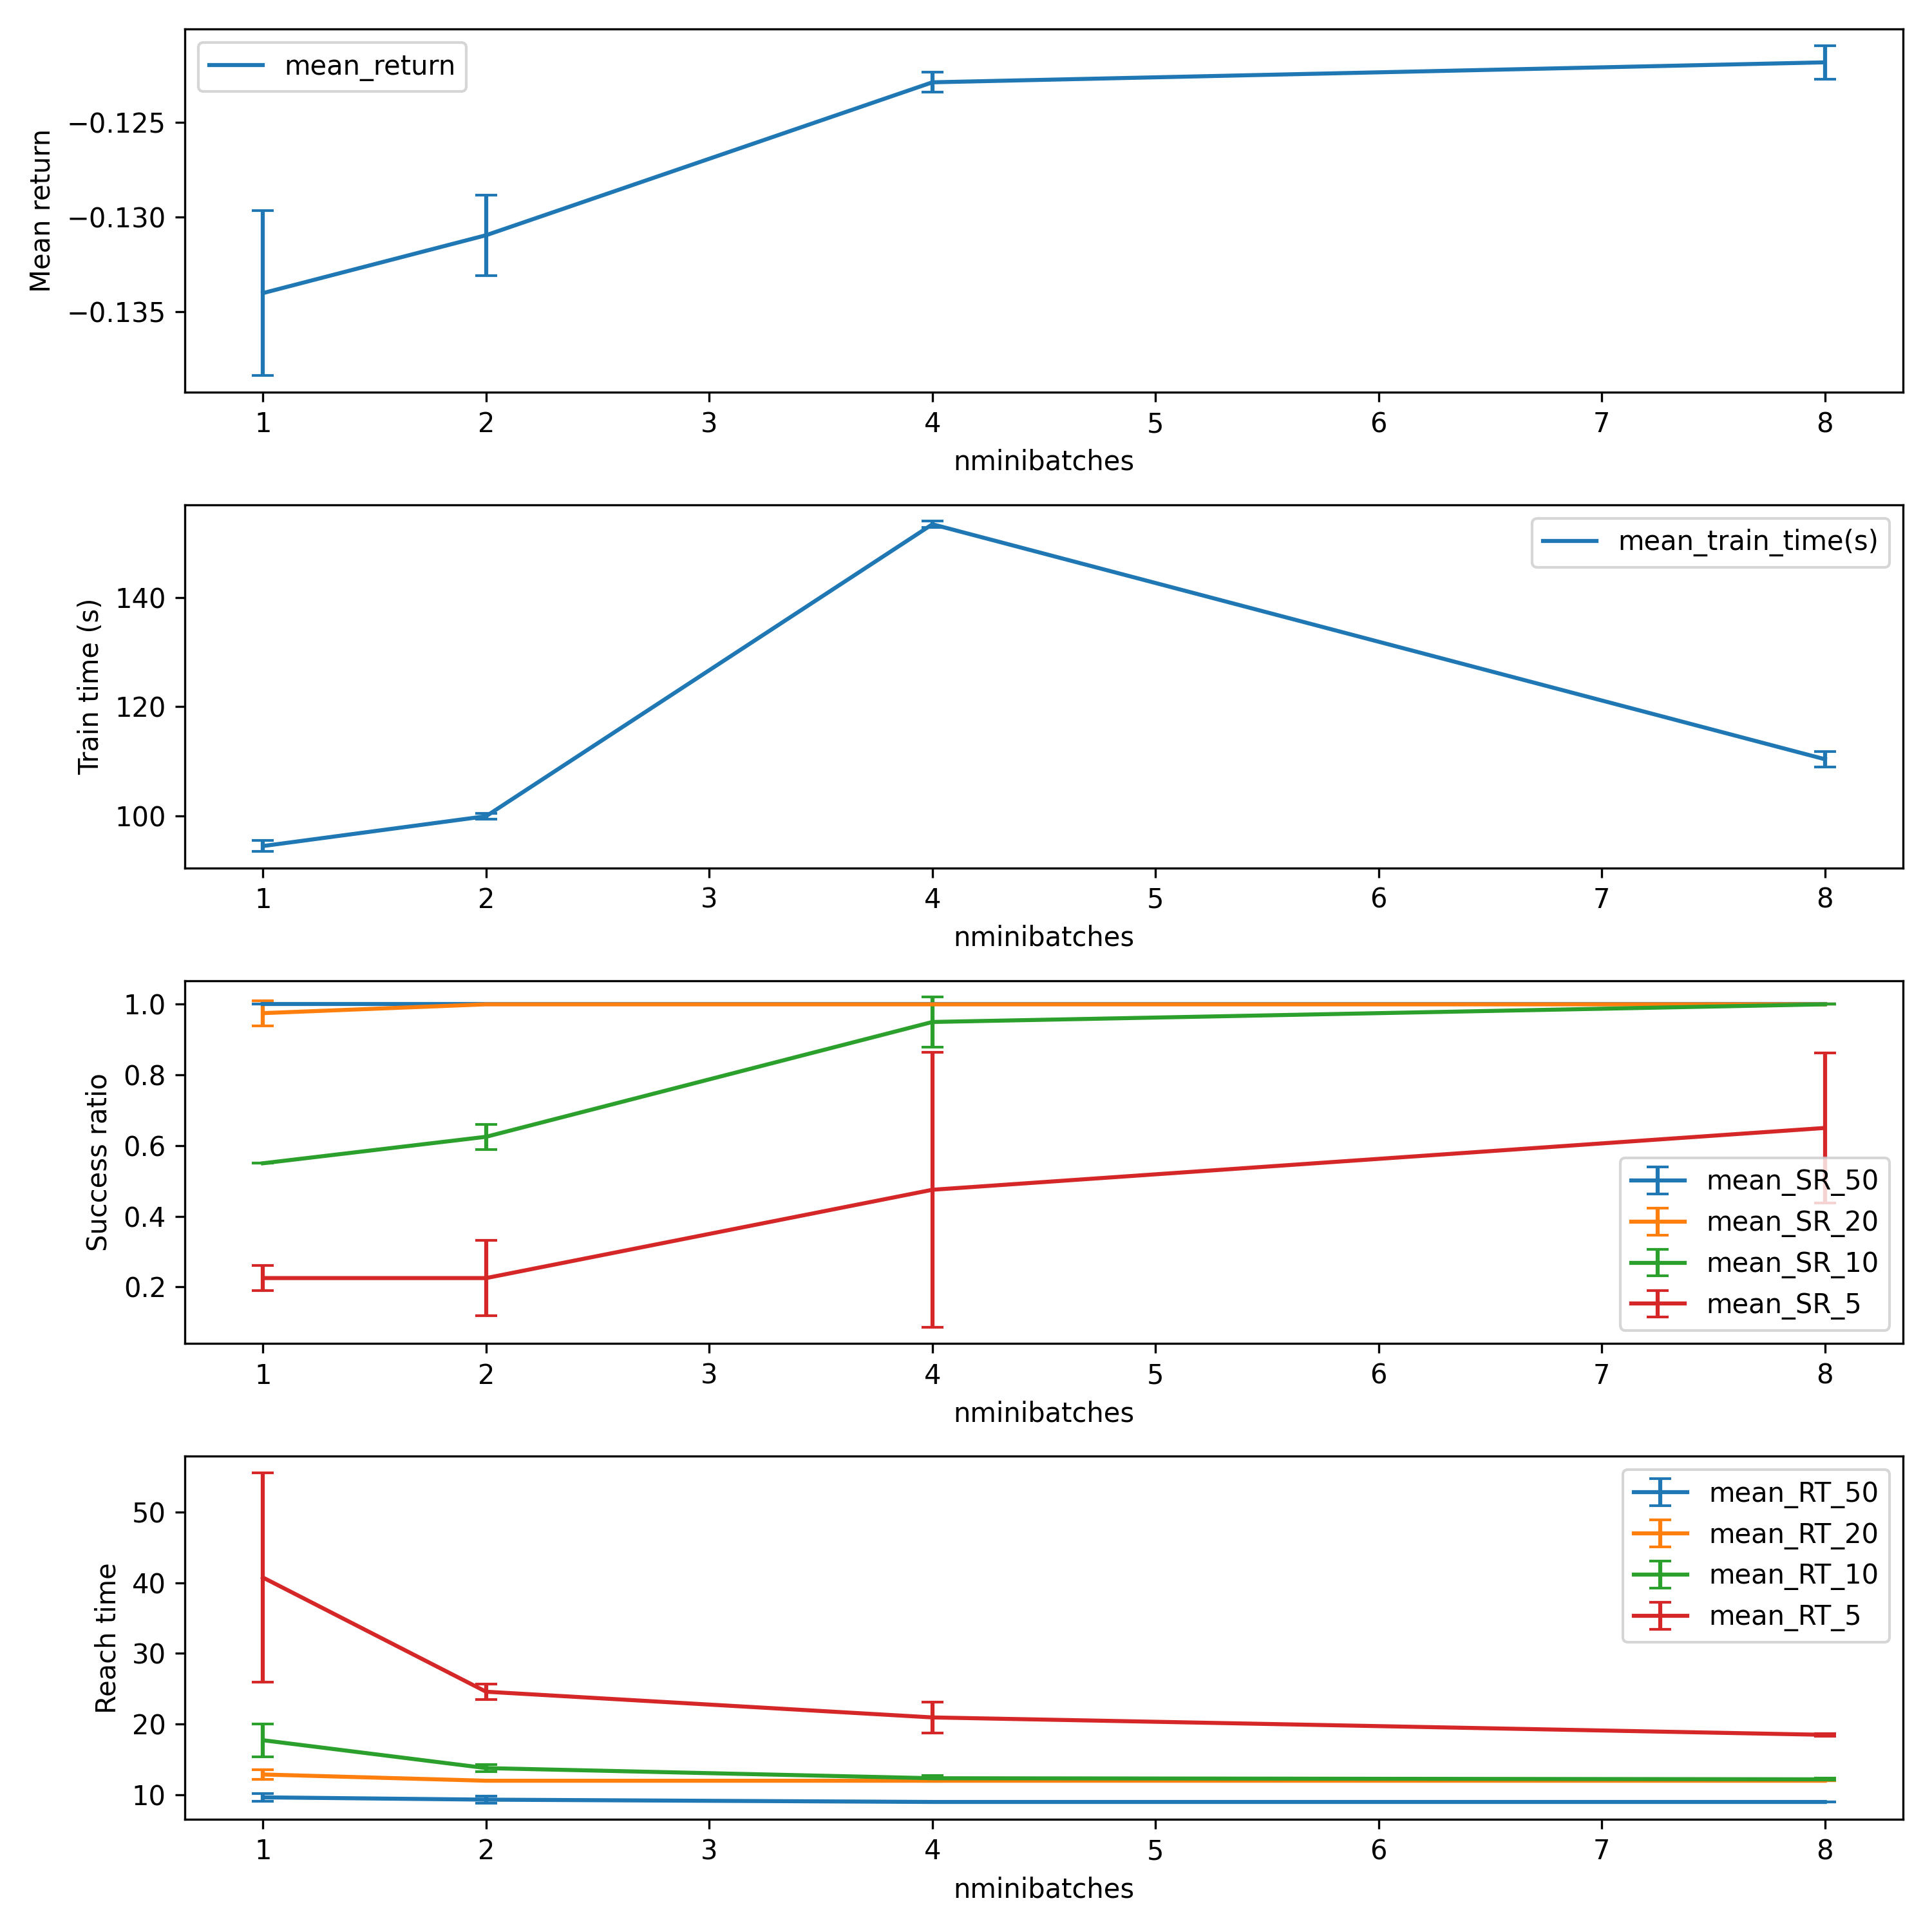
\includegraphics[width=\textwidth]{../ppo2_nminibatches.png}
\caption{Number of training minibatches per update}
\end{figure}

\begin{figure}[H]
    \centering
    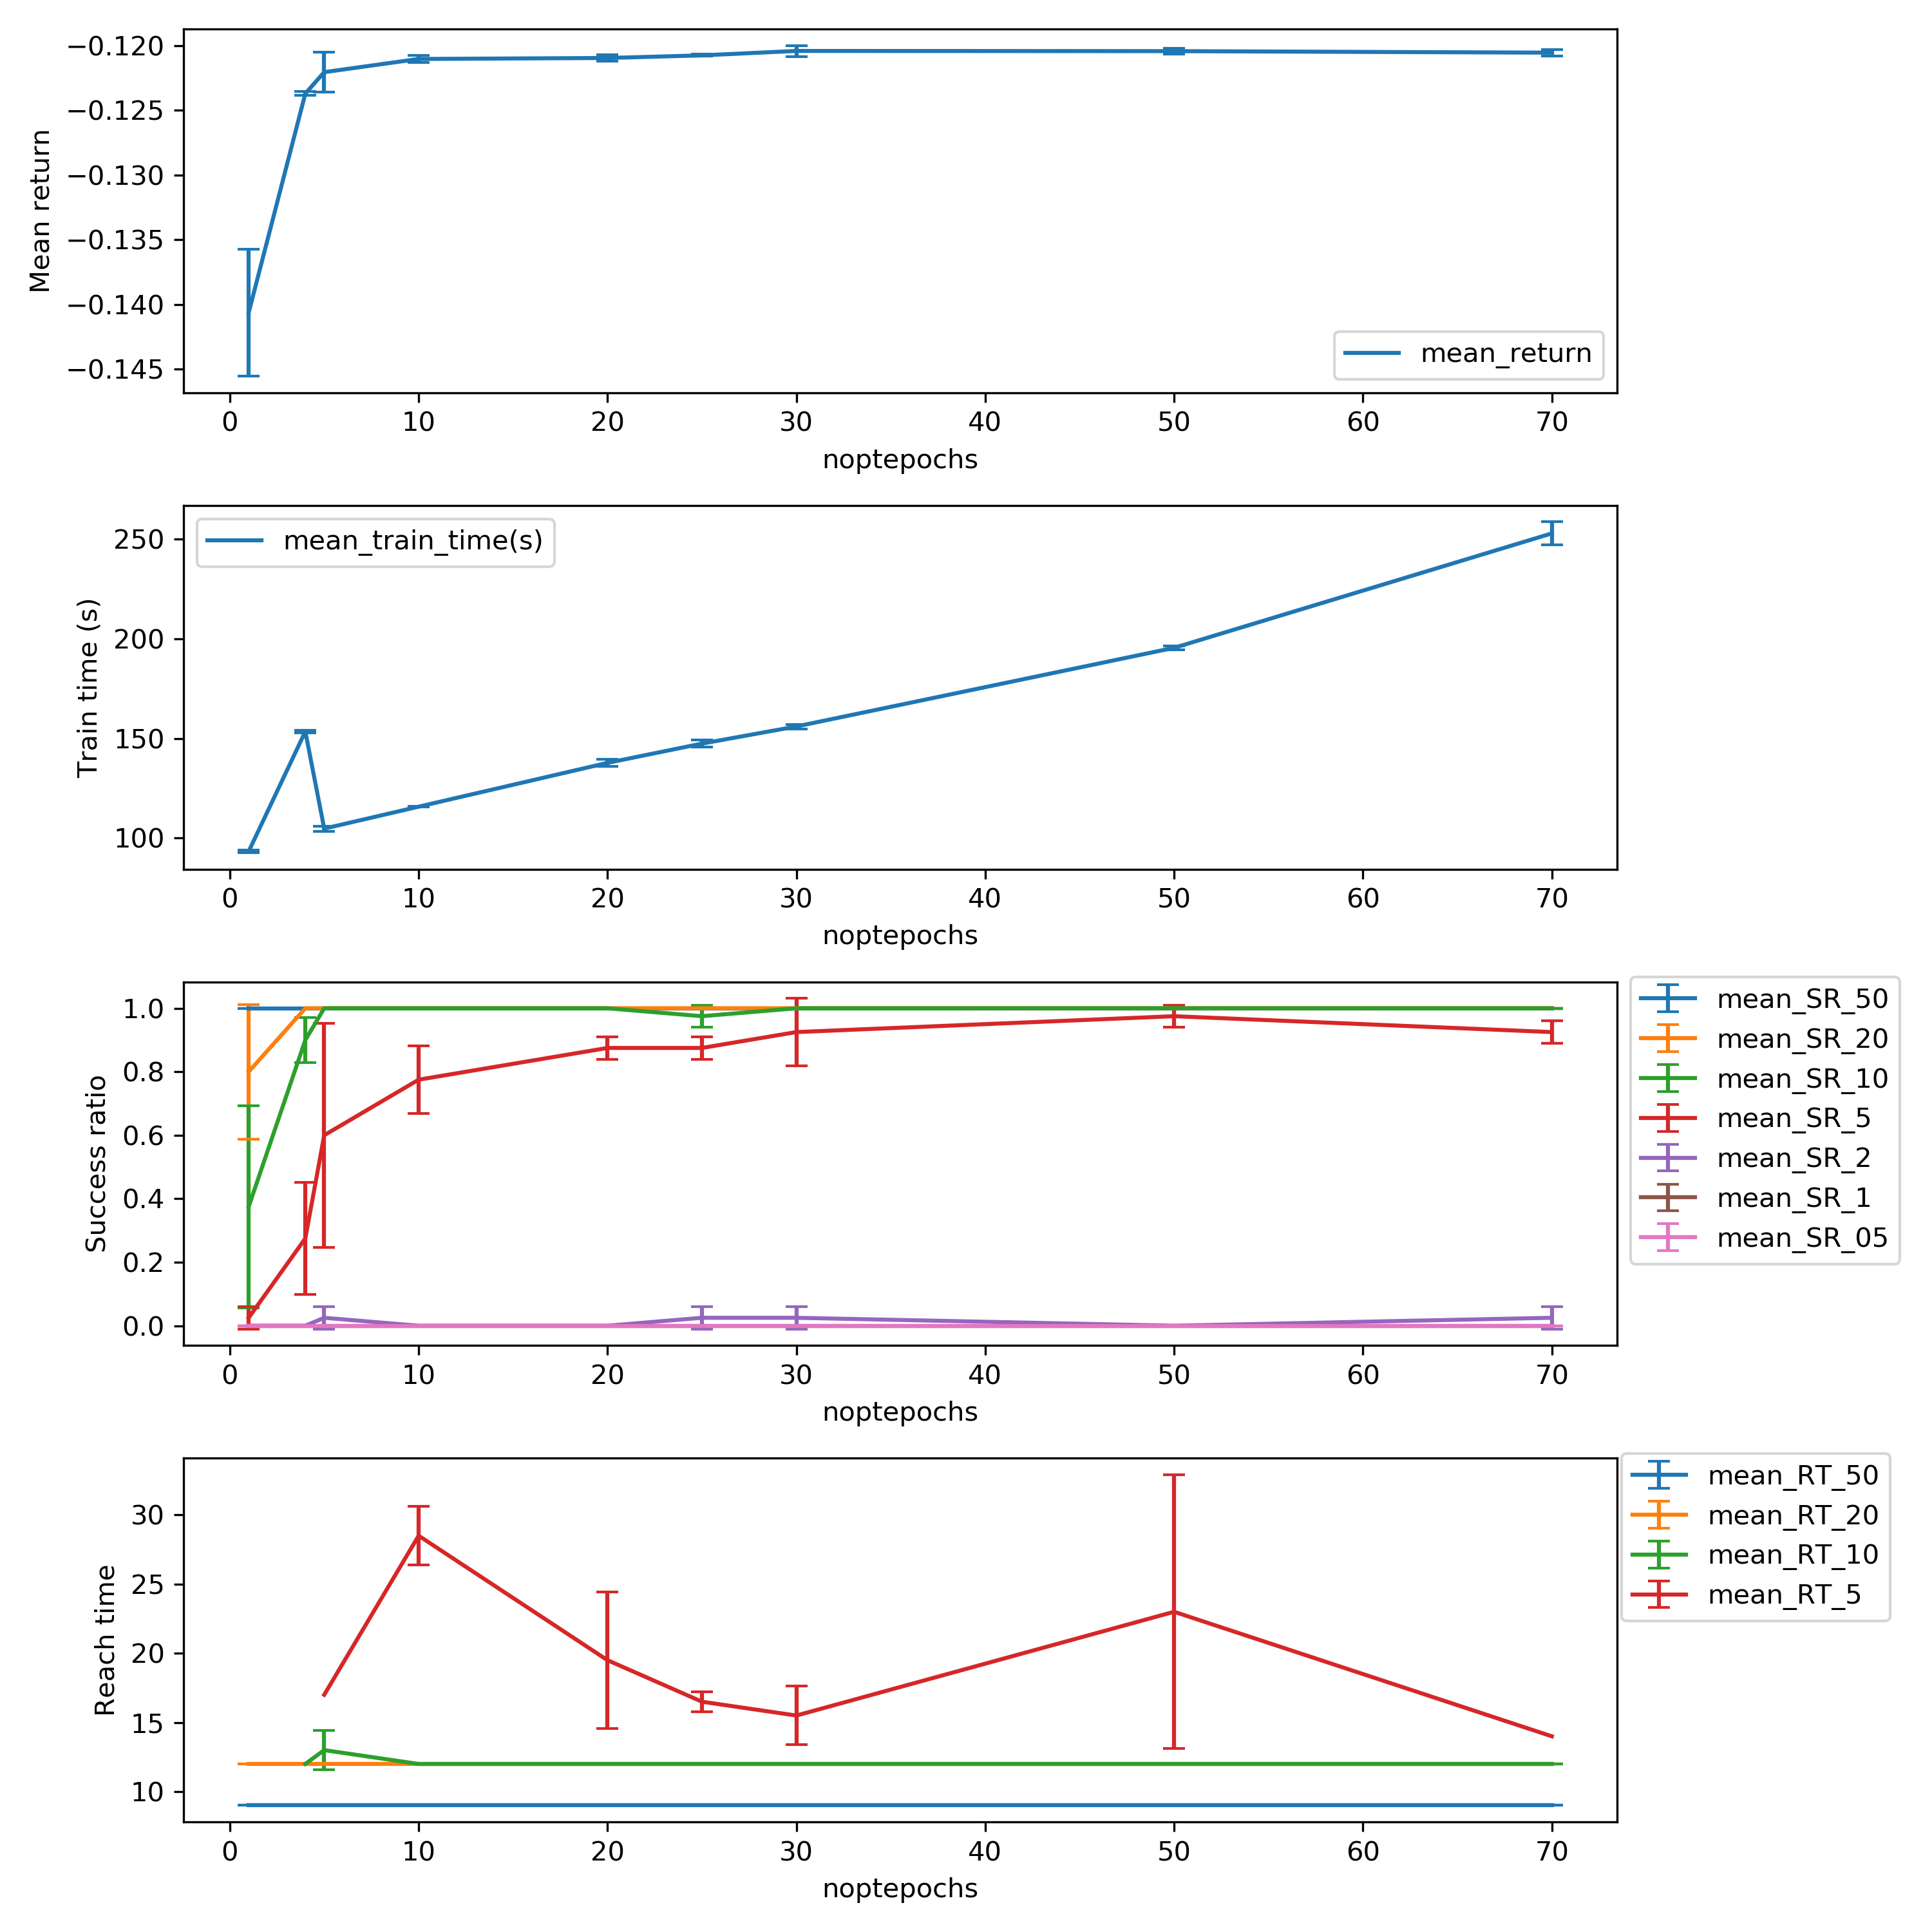
\includegraphics[width=\textwidth]{../ppo2_noptepochs.png}
\caption{Number of epoch when optimizing the surrogate}
\end{figure}



\begin{itemize}
  \item 200,000 timesteps are enough for the return to reach a plateau, however 500, 000 timesteps are required to reach the highest success ratio at 5mm. This means that the reward may not describe sufficiently well the objective we want to achieve.
  \item Best cliprange: 0.2
  \item Best ent coef: 0.01
  \item Best gamma: 0.95
  \item Best lam: 0.95 (note that the best return is not the same as the best success ration @ 5mm)
  \item Best learning rate: 0.01
  \item Best nb envs: 1 (but try also 8 since many hyperparams are fitted to this value)
  \item Best nminibatches: 8
  \item Best noptepochs: 50
  \item Best normalize: True
  \item Best nsteps: 16
\end{itemize} 


These parameters take too long to train. The best trained agent has the following parameters:

\begin{itemize}
  \item Timesteps: 500, 000
  \item cliprange: 0.2
  \item ent coef: 0.01
  \item gamma: 0.99
  \item lam: 0.95
  \item learning rate: 0.00025
  \item nb envs: 8
  \item nminibatches: 4
  \item noptepochs: 50
  \item normalize: True
  \item nsteps: 128
\end{itemize} 


\section{Environment tuning}


\begin{figure}[H]
    \centering
    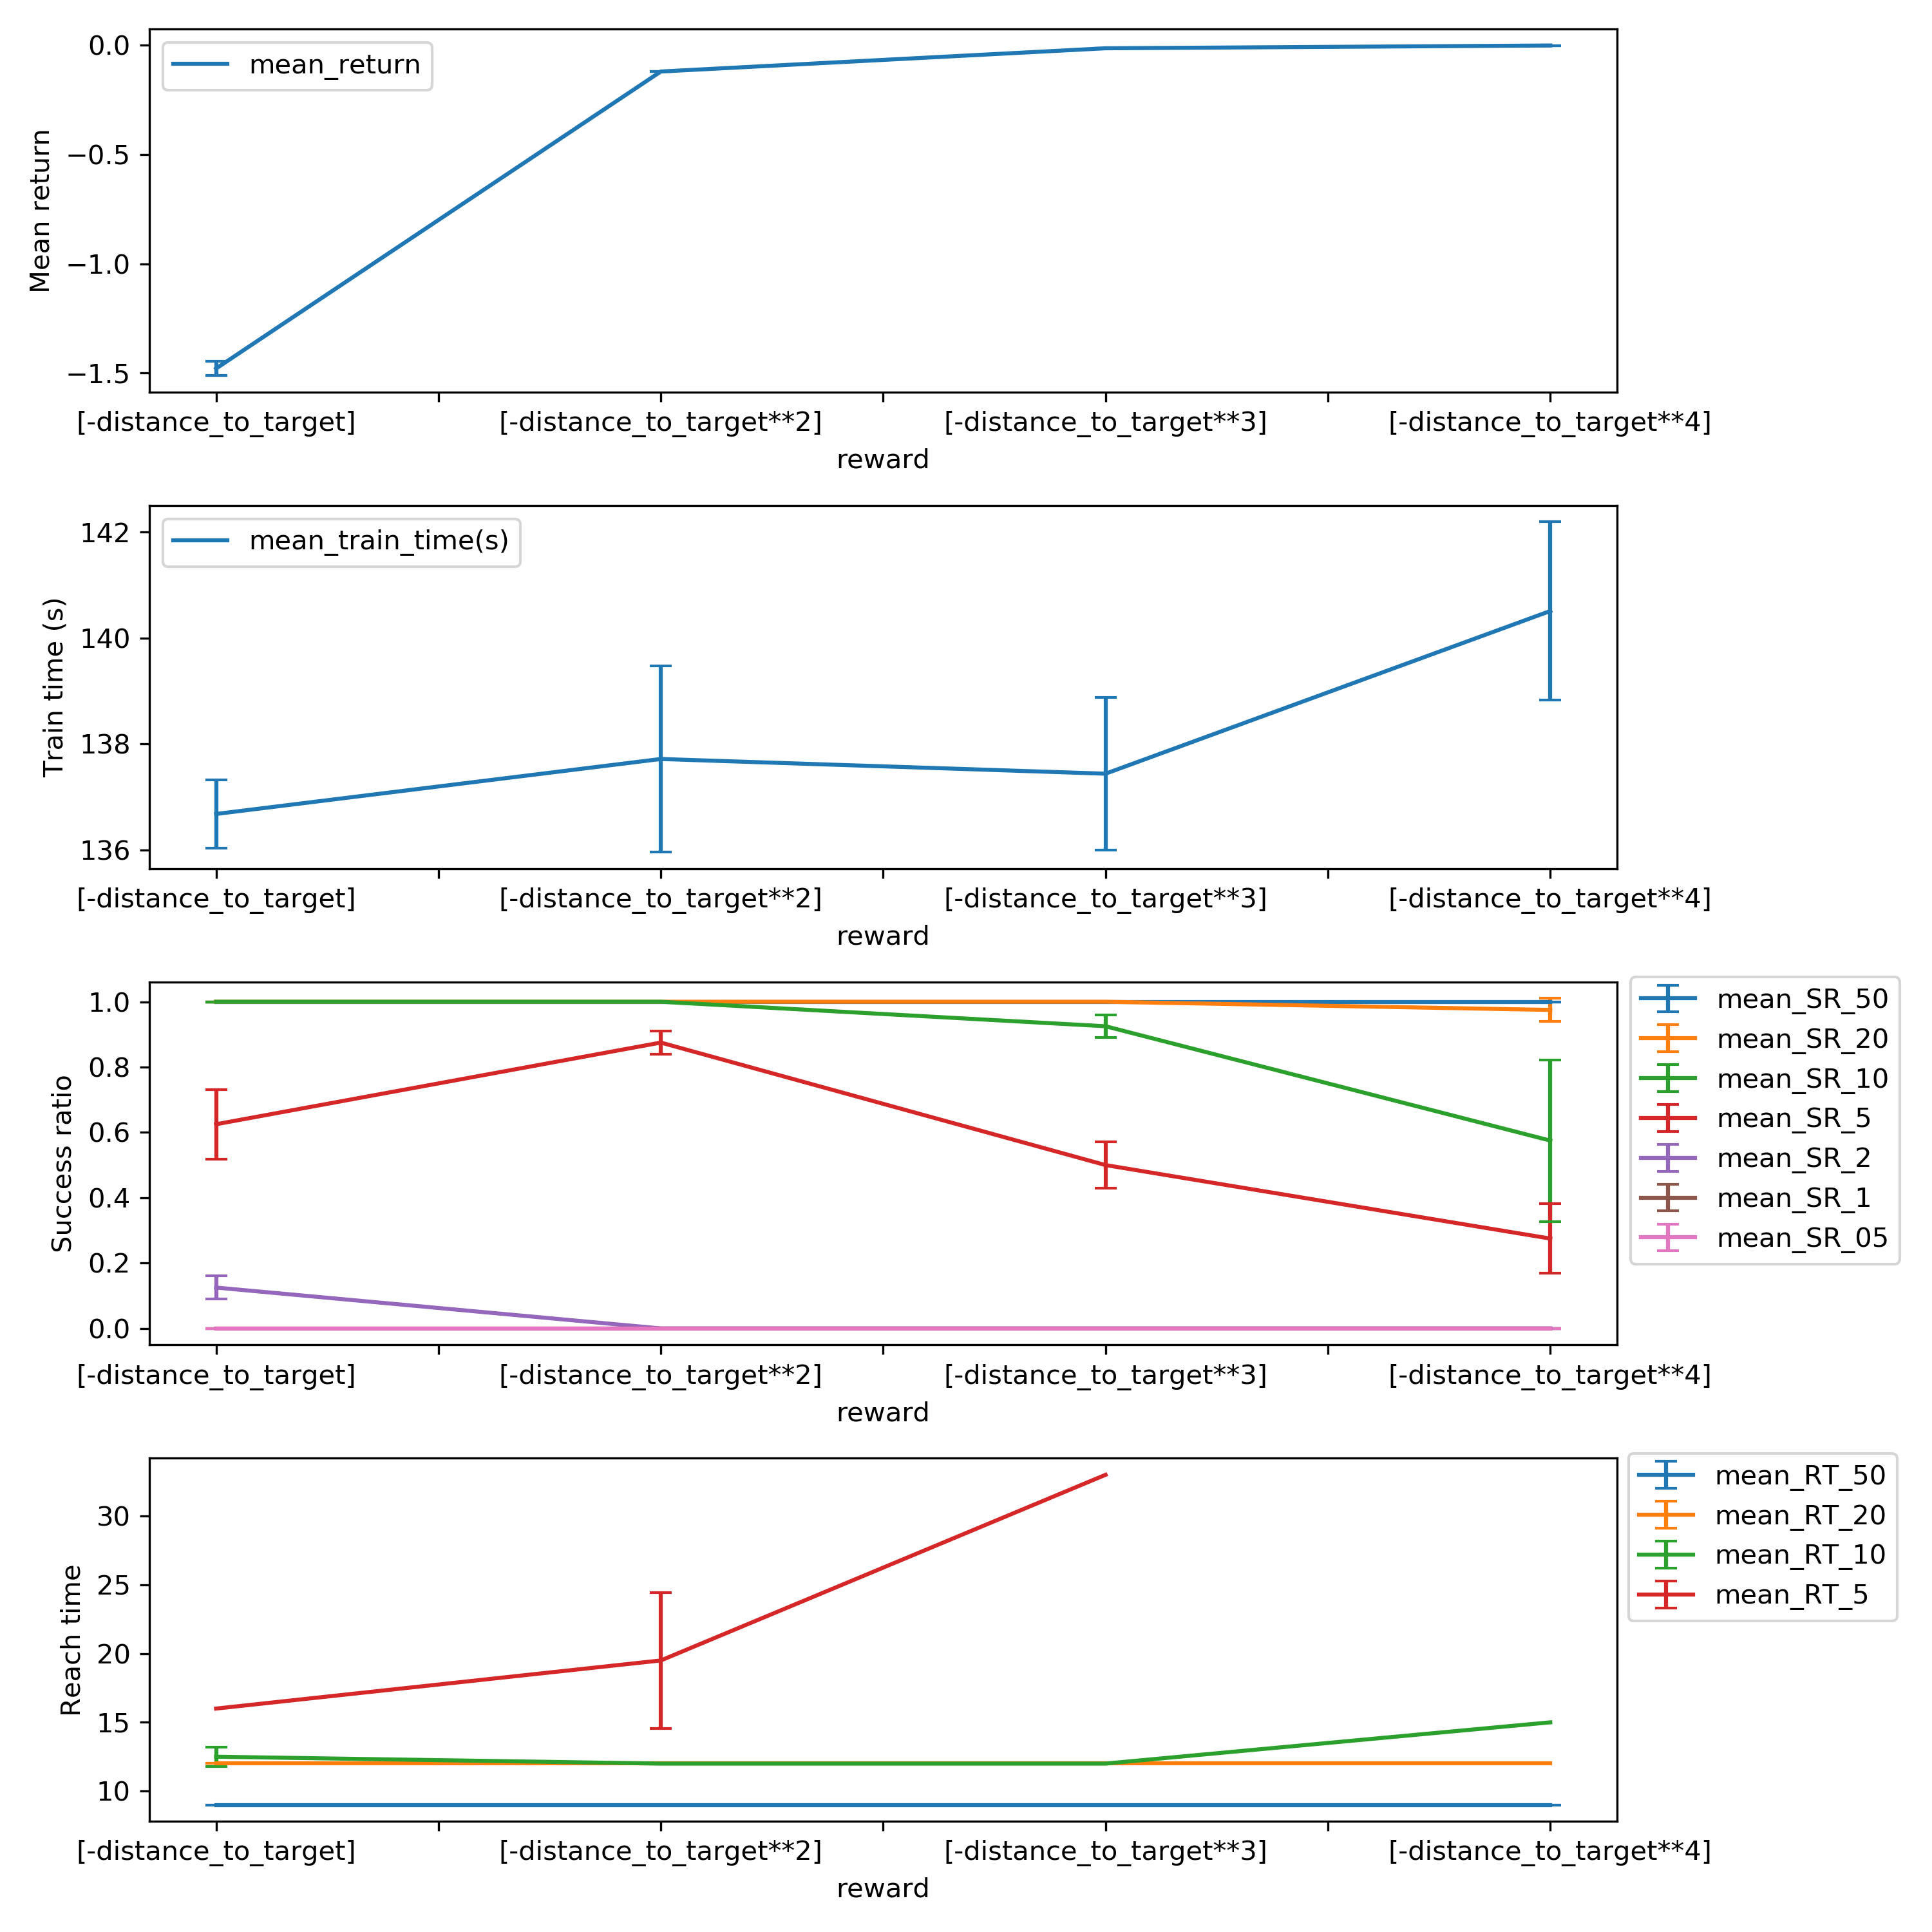
\includegraphics[width=\textwidth]{../reward_dist.png}
\caption{Reward as a function of the distance}
\end{figure}




\end{document}